\documentclass{article}
%----------------------------Preamble-------------------------------%
%---------------------------Packages----------------------------%
\usepackage{geometry}
\geometry{b5paper, margin=1.0in}
\usepackage[T1]{fontenc}
\usepackage{graphicx, float}            % Graphics/Images.
\usepackage{natbib}                     % For bibliographies.
\bibliographystyle{agsm}                % Bibliography style.
\usepackage[french, english]{babel}     % Language typesetting.
\usepackage[dvipsnames]{xcolor}         % Color names.
\usepackage{listings}                   % Verbatim-Like Tools.
\usepackage{mathtools, esint, mathrsfs} % amsmath and integrals.
\usepackage{amsthm, amsfonts, amssymb}  % Fonts and theorems.
\usepackage{tcolorbox}                  % Frames around theorems.
\usepackage{upgreek}                    % Non-Italic Greek.
\usepackage{fmtcount, etoolbox}         % For the \book{} command.
\usepackage[newparttoc]{titlesec}       % Formatting chapter, etc.
\usepackage{titletoc}                   % Allows \book in toc.
\usepackage[nottoc]{tocbibind}          % Bibliography in toc.
\usepackage[titles]{tocloft}            % ToC formatting.
\usepackage{pgfplots, tikz}             % Drawing/graphing tools.
\usepackage{imakeidx}                   % Used for index.
\usetikzlibrary{
    calc,                   % Calculating right angles and more.
    angles,                 % Drawing angles within triangles.
    arrows.meta,            % Latex and Stealth arrows.
    quotes,                 % Adding labels to angles.
    positioning,            % Relative positioning of nodes.
    decorations.markings,   % Adding arrows in the middle of a line.
    patterns,
    arrows
}                                       % Libraries for tikz.
\pgfplotsset{compat=1.9}                % Version of pgfplots.
\usepackage[font=scriptsize,
            labelformat=simple,
            labelsep=colon]{subcaption} % Subfigure captions.
\usepackage[font={scriptsize},
            hypcap=true,
            labelsep=colon]{caption}    % Figure captions.
\usepackage[pdftex,
            pdfauthor={Ryan Maguire},
            pdftitle={Mathematics and Physics},
            pdfsubject={Mathematics, Physics, Science},
            pdfkeywords={Mathematics, Physics, Computer Science, Biology},
            pdfproducer={LaTeX},
            pdfcreator={pdflatex}]{hyperref}
\hypersetup{
    colorlinks=true,
    linkcolor=blue,
    filecolor=magenta,
    urlcolor=Cerulean,
    citecolor=SkyBlue
}                           % Colors for hyperref.
\usepackage[toc,acronym,nogroupskip,nopostdot]{glossaries}
\usepackage{glossary-mcols}
%------------------------Theorem Styles-------------------------%
\theoremstyle{plain}
\newtheorem{theorem}{Theorem}[section]

% Define theorem style for default spacing and normal font.
\newtheoremstyle{normal}
    {\topsep}               % Amount of space above the theorem.
    {\topsep}               % Amount of space below the theorem.
    {}                      % Font used for body of theorem.
    {}                      % Measure of space to indent.
    {\bfseries}             % Font of the header of the theorem.
    {}                      % Punctuation between head and body.
    {.5em}                  % Space after theorem head.
    {}

% Italic header environment.
\newtheoremstyle{thmit}{\topsep}{\topsep}{}{}{\itshape}{}{0.5em}{}

% Define environments with italic headers.
\theoremstyle{thmit}
\newtheorem*{solution}{Solution}

% Define default environments.
\theoremstyle{normal}
\newtheorem{example}{Example}[section]
\newtheorem{definition}{Definition}[section]
\newtheorem{problem}{Problem}[section]

% Define framed environment.
\tcbuselibrary{most}
\newtcbtheorem[use counter*=theorem]{ftheorem}{Theorem}{%
    before=\par\vspace{2ex},
    boxsep=0.5\topsep,
    after=\par\vspace{2ex},
    colback=green!5,
    colframe=green!35!black,
    fonttitle=\bfseries\upshape%
}{thm}

\newtcbtheorem[auto counter, number within=section]{faxiom}{Axiom}{%
    before=\par\vspace{2ex},
    boxsep=0.5\topsep,
    after=\par\vspace{2ex},
    colback=Apricot!5,
    colframe=Apricot!35!black,
    fonttitle=\bfseries\upshape%
}{ax}

\newtcbtheorem[use counter*=definition]{fdefinition}{Definition}{%
    before=\par\vspace{2ex},
    boxsep=0.5\topsep,
    after=\par\vspace{2ex},
    colback=blue!5!white,
    colframe=blue!75!black,
    fonttitle=\bfseries\upshape%
}{def}

\newtcbtheorem[use counter*=example]{fexample}{Example}{%
    before=\par\vspace{2ex},
    boxsep=0.5\topsep,
    after=\par\vspace{2ex},
    colback=red!5!white,
    colframe=red!75!black,
    fonttitle=\bfseries\upshape%
}{ex}

\newtcbtheorem[auto counter, number within=section]{fnotation}{Notation}{%
    before=\par\vspace{2ex},
    boxsep=0.5\topsep,
    after=\par\vspace{2ex},
    colback=SeaGreen!5!white,
    colframe=SeaGreen!75!black,
    fonttitle=\bfseries\upshape%
}{not}

\newtcbtheorem[use counter*=remark]{fremark}{Remark}{%
    fonttitle=\bfseries\upshape,
    colback=Goldenrod!5!white,
    colframe=Goldenrod!75!black}{ex}

\newenvironment{bproof}{\textit{Proof.}}{\hfill$\square$}
\tcolorboxenvironment{bproof}{%
    blanker,
    breakable,
    left=3mm,
    before skip=5pt,
    after skip=10pt,
    borderline west={0.6mm}{0pt}{green!80!black}
}

\AtEndEnvironment{lexample}{$\hfill\textcolor{red}{\blacksquare}$}
\newtcbtheorem[use counter*=example]{lexample}{Example}{%
    empty,
    title={Example~\theexample},
    boxed title style={%
        empty,
        size=minimal,
        toprule=2pt,
        top=0.5\topsep,
    },
    coltitle=red,
    fonttitle=\bfseries,
    parbox=false,
    boxsep=0pt,
    before=\par\vspace{2ex},
    left=0pt,
    right=0pt,
    top=3ex,
    bottom=1ex,
    before=\par\vspace{2ex},
    after=\par\vspace{2ex},
    breakable,
    pad at break*=0mm,
    vfill before first,
    overlay unbroken={%
        \draw[red, line width=2pt]
            ([yshift=-1.2ex]title.south-|frame.west) to
            ([yshift=-1.2ex]title.south-|frame.east);
        },
    overlay first={%
        \draw[red, line width=2pt]
            ([yshift=-1.2ex]title.south-|frame.west) to
            ([yshift=-1.2ex]title.south-|frame.east);
    },
}{ex}

\AtEndEnvironment{ldefinition}{$\hfill\textcolor{Blue}{\blacksquare}$}
\newtcbtheorem[use counter*=definition]{ldefinition}{Definition}{%
    empty,
    title={Definition~\thedefinition:~{#1}},
    boxed title style={%
        empty,
        size=minimal,
        toprule=2pt,
        top=0.5\topsep,
    },
    coltitle=Blue,
    fonttitle=\bfseries,
    parbox=false,
    boxsep=0pt,
    before=\par\vspace{2ex},
    left=0pt,
    right=0pt,
    top=3ex,
    bottom=0pt,
    before=\par\vspace{2ex},
    after=\par\vspace{1ex},
    breakable,
    pad at break*=0mm,
    vfill before first,
    overlay unbroken={%
        \draw[Blue, line width=2pt]
            ([yshift=-1.2ex]title.south-|frame.west) to
            ([yshift=-1.2ex]title.south-|frame.east);
        },
    overlay first={%
        \draw[Blue, line width=2pt]
            ([yshift=-1.2ex]title.south-|frame.west) to
            ([yshift=-1.2ex]title.south-|frame.east);
    },
}{def}

\AtEndEnvironment{ltheorem}{$\hfill\textcolor{Green}{\blacksquare}$}
\newtcbtheorem[use counter*=theorem]{ltheorem}{Theorem}{%
    empty,
    title={Theorem~\thetheorem:~{#1}},
    boxed title style={%
        empty,
        size=minimal,
        toprule=2pt,
        top=0.5\topsep,
    },
    coltitle=Green,
    fonttitle=\bfseries,
    parbox=false,
    boxsep=0pt,
    before=\par\vspace{2ex},
    left=0pt,
    right=0pt,
    top=3ex,
    bottom=-1.5ex,
    breakable,
    pad at break*=0mm,
    vfill before first,
    overlay unbroken={%
        \draw[Green, line width=2pt]
            ([yshift=-1.2ex]title.south-|frame.west) to
            ([yshift=-1.2ex]title.south-|frame.east);},
    overlay first={%
        \draw[Green, line width=2pt]
            ([yshift=-1.2ex]title.south-|frame.west) to
            ([yshift=-1.2ex]title.south-|frame.east);
    }
}{thm}

%--------------------Declared Math Operators--------------------%
\DeclareMathOperator{\adjoint}{adj}         % Adjoint.
\DeclareMathOperator{\Card}{Card}           % Cardinality.
\DeclareMathOperator{\curl}{curl}           % Curl.
\DeclareMathOperator{\diam}{diam}           % Diameter.
\DeclareMathOperator{\dist}{dist}           % Distance.
\DeclareMathOperator{\Div}{div}             % Divergence.
\DeclareMathOperator{\Erf}{Erf}             % Error Function.
\DeclareMathOperator{\Erfc}{Erfc}           % Complementary Error Function.
\DeclareMathOperator{\Ext}{Ext}             % Exterior.
\DeclareMathOperator{\GCD}{GCD}             % Greatest common denominator.
\DeclareMathOperator{\grad}{grad}           % Gradient
\DeclareMathOperator{\Ima}{Im}              % Image.
\DeclareMathOperator{\Int}{Int}             % Interior.
\DeclareMathOperator{\LC}{LC}               % Leading coefficient.
\DeclareMathOperator{\LCM}{LCM}             % Least common multiple.
\DeclareMathOperator{\LM}{LM}               % Leading monomial.
\DeclareMathOperator{\LT}{LT}               % Leading term.
\DeclareMathOperator{\Mod}{mod}             % Modulus.
\DeclareMathOperator{\Mon}{Mon}             % Monomial.
\DeclareMathOperator{\multideg}{mutlideg}   % Multi-Degree (Graphs).
\DeclareMathOperator{\nul}{nul}             % Null space of operator.
\DeclareMathOperator{\Ord}{Ord}             % Ordinal of ordered set.
\DeclareMathOperator{\Prin}{Prin}           % Principal value.
\DeclareMathOperator{\proj}{proj}           % Projection.
\DeclareMathOperator{\Refl}{Refl}           % Reflection operator.
\DeclareMathOperator{\rk}{rk}               % Rank of operator.
\DeclareMathOperator{\sgn}{sgn}             % Sign of a number.
\DeclareMathOperator{\sinc}{sinc}           % Sinc function.
\DeclareMathOperator{\Span}{Span}           % Span of a set.
\DeclareMathOperator{\Spec}{Spec}           % Spectrum.
\DeclareMathOperator{\supp}{supp}           % Support
\DeclareMathOperator{\Tr}{Tr}               % Trace of matrix.
%--------------------Declared Math Symbols--------------------%
\DeclareMathSymbol{\minus}{\mathbin}{AMSa}{"39} % Unary minus sign.
%------------------------New Commands---------------------------%
\DeclarePairedDelimiter\norm{\lVert}{\rVert}
\DeclarePairedDelimiter\ceil{\lceil}{\rceil}
\DeclarePairedDelimiter\floor{\lfloor}{\rfloor}
\newcommand*\diff{\mathop{}\!\mathrm{d}}
\newcommand*\Diff[1]{\mathop{}\!\mathrm{d^#1}}
\renewcommand*{\glstextformat}[1]{\textcolor{RoyalBlue}{#1}}
\renewcommand{\glsnamefont}[1]{\textbf{#1}}
\renewcommand\labelitemii{$\circ$}
\renewcommand\thesubfigure{%
    \arabic{chapter}.\arabic{figure}.\arabic{subfigure}}
\addto\captionsenglish{\renewcommand{\figurename}{Fig.}}
\numberwithin{equation}{section}

\renewcommand{\vector}[1]{\boldsymbol{\mathrm{#1}}}

\newcommand{\uvector}[1]{\boldsymbol{\hat{\mathrm{#1}}}}
\newcommand{\topspace}[2][]{(#2,\tau_{#1})}
\newcommand{\measurespace}[2][]{(#2,\varSigma_{#1},\mu_{#1})}
\newcommand{\measurablespace}[2][]{(#2,\varSigma_{#1})}
\newcommand{\manifold}[2][]{(#2,\tau_{#1},\mathcal{A}_{#1})}
\newcommand{\tanspace}[2]{T_{#1}{#2}}
\newcommand{\cotanspace}[2]{T_{#1}^{*}{#2}}
\newcommand{\Ckspace}[3][\mathbb{R}]{C^{#2}(#3,#1)}
\newcommand{\funcspace}[2][\mathbb{R}]{\mathcal{F}(#2,#1)}
\newcommand{\smoothvecf}[1]{\mathfrak{X}(#1)}
\newcommand{\smoothonef}[1]{\mathfrak{X}^{*}(#1)}
\newcommand{\bracket}[2]{[#1,#2]}

%------------------------Book Command---------------------------%
\makeatletter
\renewcommand\@pnumwidth{1cm}
\newcounter{book}
\renewcommand\thebook{\@Roman\c@book}
\newcommand\book{%
    \if@openright
        \cleardoublepage
    \else
        \clearpage
    \fi
    \thispagestyle{plain}%
    \if@twocolumn
        \onecolumn
        \@tempswatrue
    \else
        \@tempswafalse
    \fi
    \null\vfil
    \secdef\@book\@sbook
}
\def\@book[#1]#2{%
    \refstepcounter{book}
    \addcontentsline{toc}{book}{\bookname\ \thebook:\hspace{1em}#1}
    \markboth{}{}
    {\centering
     \interlinepenalty\@M
     \normalfont
     \huge\bfseries\bookname\nobreakspace\thebook
     \par
     \vskip 20\p@
     \Huge\bfseries#2\par}%
    \@endbook}
\def\@sbook#1{%
    {\centering
     \interlinepenalty \@M
     \normalfont
     \Huge\bfseries#1\par}%
    \@endbook}
\def\@endbook{
    \vfil\newpage
        \if@twoside
            \if@openright
                \null
                \thispagestyle{empty}%
                \newpage
            \fi
        \fi
        \if@tempswa
            \twocolumn
        \fi
}
\newcommand*\l@book[2]{%
    \ifnum\c@tocdepth >-3\relax
        \addpenalty{-\@highpenalty}%
        \addvspace{2.25em\@plus\p@}%
        \setlength\@tempdima{3em}%
        \begingroup
            \parindent\z@\rightskip\@pnumwidth
            \parfillskip -\@pnumwidth
            {
                \leavevmode
                \Large\bfseries#1\hfill\hb@xt@\@pnumwidth{\hss#2}
            }
            \par
            \nobreak
            \global\@nobreaktrue
            \everypar{\global\@nobreakfalse\everypar{}}%
        \endgroup
    \fi}
\newcommand\bookname{Book}
\renewcommand{\thebook}{\texorpdfstring{\Numberstring{book}}{book}}
\providecommand*{\toclevel@book}{-2}
\makeatother
\titleformat{\part}[display]
    {\Large\bfseries}
    {\partname\nobreakspace\thepart}
    {0mm}
    {\Huge\bfseries}
\titlecontents{part}[0pt]
    {\large\bfseries}
    {\partname\ \thecontentslabel: \quad}
    {}
    {\hfill\contentspage}
\titlecontents{chapter}[0pt]
    {\bfseries}
    {\chaptername\ \thecontentslabel:\quad}
    {}
    {\hfill\contentspage}
\newglossarystyle{longpara}{%
    \setglossarystyle{long}%
    \renewenvironment{theglossary}{%
        \begin{longtable}[l]{{p{0.25\hsize}p{0.65\hsize}}}
    }{\end{longtable}}%
    \renewcommand{\glossentry}[2]{%
        \glstarget{##1}{\glossentryname{##1}}%
        &\glossentrydesc{##1}{~##2.}
        \tabularnewline%
        \tabularnewline
    }%
}
\newglossary[not-glg]{notation}{not-gls}{not-glo}{Notation}
\newcommand*{\newnotation}[4][]{%
    \newglossaryentry{#2}{type=notation, name={\textbf{#3}, },
                          text={#4}, description={#4},#1}%
}
%--------------------------LENGTHS------------------------------%
% Spacings for the Table of Contents.
\addtolength{\cftsecnumwidth}{1ex}
\addtolength{\cftsubsecindent}{1ex}
\addtolength{\cftsubsecnumwidth}{1ex}
\addtolength{\cftfignumwidth}{1ex}
\addtolength{\cfttabnumwidth}{1ex}

% Indent and paragraph spacing.
\setlength{\parindent}{0em}
\setlength{\parskip}{0em}
\graphicspath{{../../images/}}       % Path to Image Folder.
%----------------------------GLOSSARY-------------------------------%
\makeglossaries
\loadglsentries{../../glossary}
\loadglsentries{../../acronym}
%--------------------------Main Document----------------------------%
\begin{document}
    \title{Notes on Miscellaneous Papers}
    \author{Ryan Maguire}
    \date{\vspace{-5ex}}
    \maketitle
    \tableofcontents
    \listoffigures
    \listoftables
    \clearpage
    \section{Some Useful References}
        \begin{itemize}[itemsep=0pt]
            \item \href{https://pds-rings.seti.org/%
                        voyager/rss/index.html}
                       {Processed Data from Voyager.}
            \item \href{https://pds-rings.seti.org/volumes/%
                        VG_28xx_peer_review/VG_2803/S_RINGS/%
                        EASYDATA/DATAINFO.TXT}
                       {Description of Easy Data.}
            \item \href{https://pds-rings.seti.org/volumes/%
                        VG_28xx_peer_review/VG_2803/S_RINGS/%
                        EDITDATA/DATAINFO.TXT}
                       {Description of data files that include%
                        diffraction and diffraction-corrected%
                        data.}
            \item \href{https://pds-rings.seti.org/volumes/%
                        VG_28xx_peer_review/VG_2803/S_RINGS/%
                        EDITDATA/RS1D1XUI.LBL}
                       {Uncorrected files from Voyager.}
            \item \href{https://pds-rings.seti.org/volumes/%
                        VG_28xx_peer_review/VG_2803/S_RINGS/%
                        GEOMETRY/GEOMINFO.TXT}
                       {Information about converting between
                        time and ring plane radius.}
            \item \href{https://pds-rings.seti.org/holdings/%
                        volumes/COVIMS_8xxx_lien_resolution/%
                        COVIMS_8001/DOCUMENT/%
                        Occultation_Keywords.pdf}
                       {Ring Occultation Keywords.}
            \item \href{https://naif.jpl.nasa.gov/pub/%
                        naif/pds/data/co-s_j_e_v-spice-6-v1.0/%
                        cosp_1000/data/pck/pckinfo.txt}
                       {Table of geometry files in Cassini
                        SPICE archive. Contains .bsp files.}
        \end{itemize}
    \section{Cassini Radio Science User's Guide}
        \label{sec:usrguide}
        \subsection{Cassini Radio Science}
            \label{subsec:usr_cassini_radio_science}
            This guide describes \gls{rs} observations made
            by the \gls{cassini} Spacecraft, as well
            as \gls{solar corona}, \gls{relativity},
            \gls{gw} data, and descriptions of the
            \gls{huygens} landing on \gls{titan}. The types
            of data that were collected, processed and
            delivered to the \gls{nasa} \gls{pds} can be
            found \href{http://pds-atmospheres.nmsu.edu/}{here}.
            \gls{rs} data from the Huygens descent to,
            and landing on, the surface of Titan can be found
            in the \gls{esa} \gls{psa}
            \href{https://www.cosmos.esa.int/?%
                  project=PSA&page=huygens}{here}.
            Appendices can be found
            \href{https://radioscience.jpl.nasa.gov/%
                  publications/index.html}{here}.
            Cassini-Huygens launched October 15, 1997 and had
            five phases: \Gls{cruise mission} ($1997\!-\!2004$),
            \gls{prime mission} ($2004\! -\! 2008$),
            \gls{equinox mission} ($2008\! -\! 2010$),
            \gls{solstice mission} ($2010\! -\! 2016$),
            \gls{grand finale} ($2016\! - \!2017$).
            Arrival occured on July 1, 2004. Huygens
            released December 25, 2004 and landed on Titan
            January 14, 2005. The period following insertion
            is called the \gls{saturn tour}.
            \gls{rs} observations occurred in every phase.
            \subsubsection{Radio Science Observations
                           and Instrumentation}
                \label{subsubsec:usr_rad_sci_obs_and_inst}
                \begin{wrapfigure}[11]{l}{0.51\textwidth}
                    \centering
                    \captionsetup{type=figure}
                    \subimport{../../tikz/}
                              {Atmospheric_Occultation}
                    \caption{Refraction via an 
                             Atmospheric Occultation}
                    \label{fig:usr_planet_occ_1}
                \end{wrapfigure}
                \gls{rs} is the study of physical objects and
                phenomena using \gls{radio waves}.
                Observables include the time, \gls{amplitude},
                \gls{frequency}, \gls{phase}, and
                \gls{polarization} of a received signal.
                \gls{rs} experiments involve \gls{gravitation}
                and \gls{propagation}. Cassini served as a
                point-mass probe within the gravity field
                of \gls{saturn} and its satellites, precision
                measurements of the Earth-Cassini distance
                and \gls{relative velocity} can be used to
                infer the target body mass and higher order
                field components. \Gls{propagation} experiments
                used \glspl{occultation} to study planetary
                \glspl{ionosphere}, \glspl{neutral atmosphere},
                \gls{planetary rings}, \gls{solar plasma},
                \gls{cometary comae}, etc. During a planetary
                \gls{occultation} the spacecraft transmitted
                a signal that was
                \glslink{refraction}{refracted} by the
                target atmosphere and then received on Earth
                by the \gls{dsn}, as shown in figure
                \ref{fig:usr_planet_occ_1}. As the spacecraft
                moved, the signal probed deeper into the
                atmosphere until it was absorbed by the planet.
                The figure depicts a one-way \gls{downlink}
                observation. A \gls{one-way observation}
                involves a \gls{downlink} spacecraft-to-Earth
                signal, but no \gls{uplink} Earth-to-spacecraft
                signal. Stability of the signal depends on the
                reference \gls{oscillator} on the spacecraft;
                Cassini used an \gls{uso}.
                A \gls{two-way observation} involves a
                \gls{downlink} spacecraft-to-Earth signal
                and an \gls{uplink} Earth-to-spacecraft signal
                that is used to control the frequency of the
                \gls{downlink} signal. This provides better
                stability due to Earth's atomic clocks. The
                Earth-spacecraft line-of-sight often contained
                rings and objects that would distort the signal,
                making \glslink{one-way observation}{one-way}
                mode preferable. \Glspl{three-way observation}
                use two ground stations and the spacecraft.
                One station transmits a signal to the
                spacecraft and another receives the signals
                sent from the spacecraft. This was used when
                an observation occurred over a period of time
                that would cause one ground station to be
                blocked from view of the spacecraft.
                \glslink{three-way observation}{Three-way} 
                \begin{figure}[H]
                    \centering
                    \captionsetup{type=figure}
                	\includegraphics[%
                	    page=15,
                	    trim={1.4cm 1.25in 1.25in 1.08in},
                	    clip,
                	    width=0.49\textwidth
                    ]{images.pdf}
                    \hfill
                    \includegraphics[%
                        page=14,
                        trim={1.4cm 1.25in 1.25in 1.08in},
                        clip,
                        width=0.49\textwidth
                    ]{images.pdf}
                	\caption{%
                	    DSN Elevation maps Rev 280 and Rev 282
                    }
                	\label{fig:usr_dsn_elav_map_1}
                \end{figure}
                observations were necessary for Cassini due to the
                $68-84$ minute light travel time from Earth to
                Saturn. As shown in figure
                \ref{fig:usr_dsn_elav_map_1}, often times $2$ or
                $3$ \gls{dsn} stations were needed to complete an
                observation. Figure \ref{fig:usr_dsn_map_1} shows
                where the various \gls{dsn} stations are.
                \Gls{occultation} observations allow for
                \glslink{temperature-pressure profile}
                        {temperature-pressure}
                and \glspl{absorption profile} of
                \glspl{neutral atmosphere},
                \glspl{electron density profile} of
                \glspl{ionosphere}, and \gls{optical depth}
                and \gls{particle size distribution} profiles
                of rings to be made. Most measurements were
                wavelength dependent and some included
                \gls{polarization} effects. During close
                encounters the spacecraft antenna was deflected
                from the Earth direction to point at Saturn's
                surface or ring plane. These
                \glslink{one-way observation}{one-way}
                \gls{bsr} experiments required high
                \glspl{sampling rate} and yielded dielectric
                constants of target surfaces and size
                distributions for ring particles. \gls{gwe}
                near \glspl{solar opposition} and \gls{sce}
                were conducted during
                \glslink{cruise mission}{cruise}.
                Changes in the Earth-Cassini distance and
                \gls{relative velocity} could indicate passage
                of gravitational waves through the space
                between Earth and Cassini.
                \glslink{two-way observation}{Two-way} mode
                was used for high stability. During
                \glspl{occultation} by the sun \glspl{sce}
                investigated the \gls{solar corona}.
                \Glspl{two-way observation} were made for
                large solar radii, \glspl{one-way observation}
                for smaller solar radii and higher solar
                activity. Short radio \glspl{wavelength} are
                least affected by \gls{solar plasma}, and
                multiple \gls{wavelength} measurements yield
                total \gls{electron} content along the
                \gls{radio path}.
            \subsubsection{Spacecraft}
                \label{subsubsec:usr_spacecraft}
                Cassini was comprised of four primary modules:
                \gls{hga}, two equipment modules, and a
                propulsion module. These contained various
                subsystems, including $12$ science instruments.
                Three \gls{rtg} were mounted in the equipment
                modules; an external boom for the magnetometer
                was attached to the \gls{uem}.
            \subsubsection{%
                \footnotesize{Radio Frequency Subsystem}
            }
                \label{subsubsec:usr_rad_freq_subsys}
                \begin{wrapfigure}[16]{r}{0.5\textwidth}
                	\centering
                	\vspace{-5ex}
                	\includegraphics[%
                	    page=16,
                	    trim={1.15in 4.1in 1.15in 2.15in},
                	    clip,
                	    width=0.5\textwidth
                    ]{images.pdf}
                	\caption{Map of DSN stations}
                	\label{fig:usr_dsn_map_1}
                \end{wrapfigure}
                The \gls{rfs} provided communications to the
                \gls{dsn} and a signal source for \gls{rs}
                measurements. \gls{rs}-only components called
                the \gls{rfis} are here considered to fall within
                the \gls{rfs}. It included a pair of redundant
                \gls{x-band} \glspl{transponder} for reception
                and transmission, an \gls{s-band}
                \gls{transmitter}, and a \gls{ka-band}
                \gls{transmitter}. The \gls{uso} provided
                on-board time and \gls{frequency} reference until
                it failed in 2011. A \gls{kat}, which received
                at 34 GHz and transmitted
                \glslink{coherent}{coherently} at 32 GHz,
                supported
                \glslink{relativity}{general relativity}
                observations during the
                \glslink{cruise mission}{cruise}, but failed
                during insertion into Saturn's orbit. The
                \gls{rfs} produced an \gls{x-band} \gls{carrier}
                \glslink{modulation}{modulated} with data
                received from the \gls{cds}, amplified the
                \glslink{modulation}{modulated} carrier, and
                delivered the signal stream to the antenna
                subsystem for transmission to Earth. It also
                received and \glslink{demodulation}{demodulated}
                \gls{x-band} commands from the ground via the
                antenna subsystem. Saturn lies between 8.2
                \gls{au} and 10.2 \gls{au} throughout the year,
                creating one-way travel times of $68-84$ minutes.
                Commands from Earth could be received at $1,000$
                \gls{bps} by the \gls{hga}, and data could be
                transmitted to Earth at rates ranging from
                14,220-165,900 \gls{bps}. Data could be
                recorded on the solid state recorders for $15$
                hours while the \gls{hga} was not pointed at
                Earth, then they were played back for nine
                hours. About one gigabit of data could be
                returned each day via a 34m \gls{dsn}
                antenna; nearly four times that via a 70m
                ground antenna. The two redundant recorders
                could record and read out nearly 2 gigabits
                of data simultaneously. The \gls{cds} handled
                combined data rates in excess of 430,000
                \gls{bps} from the instruments while carrying
                on its functions of command and control.
                Since \gls{rs} observables were generated at
                the \gls{dsn}, little \gls{tlm} was of interest
                to \gls{rs}.
                \begin{table}[H]
                    \centering
                    \captionsetup{type=table}
                    \caption{Cassini RS Bands and Wavelengths}
                    \label{tab:usr_band_wav}
                    \footnotesize
                    \begin{tabular}{|c|c|c|c|}
                        \hline
                        Band&Wavelength (cm)
                        &Frequence Uplink (MHz)
                        &Frequence Downlink (MHz) \\
                        \hline
                        S&13& N/A&2298\\
                        X&3.6&7175&8425\\
                        Ka&0.9&34316&32028\\
                        \hline
                    \end{tabular}
                \end{table}
                The antenna subsystem included the 4m diameter
                \gls{hga} reflector (Which was also used for
                sun shading in the early
                \glslink{cruise mission}{cruise} phase),
                and two \glspl{lga}. All antennas operated
                at \gls{x-band}, and only the \gls{hga}
                operated at \glslink{s-band}{S},
                \glslink{ka-band}{Ka}, \glslink{x-band}{X},
                and \glslink{ku-band}{Ku} bands.
                The \gls{x-band} was used for communications,
                navigations, and \gls{rs};
                the \glslink{s-band}{S} and
                \glslink{ka-band}{Ka} bands were solely for
                \gls{rs}, and the \gls{ku-band} components were
                for the Cassini \glslink{radar}{RADAR}.
                Table \ref{tab:usr_band_wav} lists the
                various bands and wavelengths which \gls{rs}
                on Cassini used.
            \subsubsection{\footnotesize{USO}}
                \label{subsubsec:usr_USO}
                \begin{table}[H]
                    \centering
                    \captionsetup{type=table}
                    \caption{Allen Deviation for Cassini}
                    \label{tab:Allen_Deviation_for_Cassini}
                    \begin{tabular}{|c|c|}
                        \hline
                        Integration Time (s)&Allen Deviation\\
                        \hline
                        1&7.588367324486e-13\\
                        10&1.087943735011e-13\\
                        100&9.344696016571e-13\\
                        1000&2.603035874178e-13\\
                        \hline
                    \end{tabular}
                \end{table}
                The \gls{uso} provided the highly stable
                reference generated on-board the spacecraft
                until its failure in $2011$. The Cassini
                oscillator was in the class of high performance
                thermally-controlled quartz crystal oscillators
                flown on planetary missions. It was manufactured
                at the Johns Hopkins University Applied Physics
                Laboratory. In figure
                \ref{tab:usr_uso_freq_vals} we see the
                \gls{x-band} output frequency of the \gls{uso}
                over several years and can see long-term aging
                behavior
                (Without accounting for time dilation effects).
                In table \ref{tab:Allen_Deviation_for_Cassini}
                we see that the \gls{allen deviation} for the
                \gls{uso} was excellent. In reality this data
                characterizes the end-to-end performance of
                the radio systems on both the spacecraft and
                ground station, although independent
                calibration of \gls{dsn} stations have shown
                that these results are dominated primarily by
                the limit of the \gls{uso} performance.
                The stability of the \gls{uso} and the small
                \gls{allen deviation} values allow for
                \glslink{resolution}{high-resolution} ring
                profiles to be made, as is discussed in
                chapter INSERT REFERENCE CHAPTER HERE,
                section INSERT REFERENCE SECTION HERE.
                It can be shown, all other factors held
                constant, that the resolution depends on the
                \gls{allen deviation} as follows:
                \begin{equation}
                    R_{res}\propto
                    \frac{\sigma_{t}^{2}}
                         {\exp{-a\sigma_{t}}+a\sigma_{t}-1}
                \end{equation}
                Where $\sigma_{t}$ is the \gls{allen deviation}
                corresponding to $t$-seconds of integration
                time and $a$ depends on the frequency $f$ and
                the geometry of the spacecraft.
                \begin{table}[H]
                    \centering
                    \captionsetup{type=table}
                    \caption{USO Frequency $2006-2011$}
                    \label{tab:usr_uso_freq_vals}
                    \begin{tabular}{|ccccc|ccccc|}
                        \hline
                        Day&Frequency (Hz)&Year&DOY
                            &&&Day&Frequency (Hz)&Year&DOY\\
                        \hline
                        51&8427222036.34067&2006&51
                            &&&526&8427222041.35297&2007&161\\
                        76&8427222036.52366&2006&76
                            &&&632 &8427222041.49555&2007&267\\
                        78&8427222036.20419&2006&78
                            &&&712 &8427222041.63084&2007&347\\
                        110&8427222036.42800&2006&110
                            &&&829 &8427222042.31336&2008&99 \\
                        123&8427222034.34050&2006&123
                            &&&908 &8427222041.00434&2008&178\\
                        126&8427222043.98074&2006&126
                            &&&937 &8427222040.45283&2008&207\\
                        134&8427222043.25770&2006&134
                            &&&989 &8427222040.90144&2008&259\\
                        141&8427222034.29712&2006&141
                            &&&1032&8427222041.27468&2008&302\\
                        159&8427222034.62180&2006&159
                            &&&1124&8427222042.84108&2009& 28\\
                        178&8427222034.66356&2006&178
                            &&&1155&8427222043.14919&2009& 59\\
                        196&8427222034.83532&2006&196
                            &&&1249&8427222043.48567&2009&153\\
                        214&8427222034.92818&2006&214
                            &&&1327&8427222044.16133&2009&232\\
                        232&8427222035.09925&2006&232
                            &&&1465&8427222045.42919&2010&  4\\
                        242&8427222041.00252&2006&242
                            &&&1568&8427222046.85504&2010&107\\
                        248&8427222033.76827&2006&248
                            &&&1607&8427222047.34145&2010&146\\
                        260&8427222041.02353&2006&260
                            &&&1747&8427222049.43250&2010&286\\
                        320&8427222041.37934&2006&320
                            &&&1845&8427222050.84059&2011& 19\\
                        353&8427222041.70860&2006&353
                            &&&1943&8427222052.16839&2011&117\\
                        356&8427222041.74006&2006&356
                            &&&2028&8427222053.08372&2011&202\\
                        393&8427222042.06867&2007&28
                            &&&2151&8427222055.29388&2011&325\\
                        436&8427222042.17835&2007&71
                            &&&2170&8427222055.69421&2011&345\\
                        \hline
                    \end{tabular}
                \end{table}
            \subsubsection{%
                \footnotesize{%
                    Attitude and Articulation
                    Control Subsystem
                }
            }
                \label{subsubsec:usr_att_and_art_cont_subsye}
                The \gls{aacs} maintained the spacecraft's
                orientation and consisted of redundant sun
                sensors mounted on the \gls{hga}, redundant
                stellar reference units mounted on the
                remote-sensing platform, three mutually
                perpendicular reaction wheels mounted in the
                \gls{lem}, and a fourth backup wheel mounted in
                the \gls{uem}. The \gls{aacs} pointed the selected
                communication antenna towards Earth and pointed
                the remote sensing pallet towards the selected
                target. It also pointed one of the two redundant
                main propulsion engines in the desired direction
                during engine burns and performed small trajectory
                correction maneuvers using the on-board thrusters.
                The \gls{aacs} used a pointing system known as
                \gls{inertial vector propagation} that kept track
                of spacecraft orientation, the direction of the
                Sun, and distance to the Sun, Earth, Saturn,
                and other remote sensing targets, and the
                spacecraft-relative pointing directions of all
                science instruments.
            \subsubsection{\footnotesize{Other Subsystems}}
                \label{subsubsec:usr_other_subsys}
                The \gls{pms} was the target subsystem. It
                consisted of a bi-propellant element for
                trajectory changes and a \gls{hydrazine} element
                for attitude control, small maneuvers, and
                reaction wheel desaturation. The \gls{pps}
                converted the \gls{rtg} power output to provide
                a regulated 30-V \gls{dc} power bus and provided
                the capability to turn various users on or off
                when commanded. The \gls{tcs} maintained the
                temperatures of all critical spacecraft
                components. Even at $9$ \gls{au}, exposing
                radiator plates to the Sun could severely degrade
                the data collected by science instruments. The
                \gls{tcs} could turn electric heaters on or off,
                open or shut thermal louvers in the \gls{uem},
                use small radioisotope heaters, and use thermal
                blankets and shields.
            \subsubsection{\footnotesize{Ground Systems}}
                \label{subsubsec:usr_ground_sys}
                RS data was acquired by \gls{dsn} stations in
                Goldstone, California; Canberra, Australia;
                and Madrid, Spain
                (See Fig~\ref{fig:usr_dsn_map_1}),
                where both 34m and 70m antennas were used.
                Antennas were fixed to lower frequencies when
                sampled, averaged, and recorded for later
                analysis. Ground stations were pointed via
                several different techniques. \Glspl{conical scan}
                used dynamical ground antenna pointing during
                which the boresight is offset from the predicted
                pointing by a small amount. The observed
                degradation in signal level was used to determine
                a new pointing direction. This was not used when
                the signal is expected to undergo significant
                amplitude changes. \Gls{monopulse} used relative
                amplitude and phase between $TE_{11}$ and
                $TE_{12}$ circular \gls{waveguide} mode signals
                generated in a special \gls{ka-band} feed.
                \Gls{aberration correction} used a pointing
                adjustment to account for the real motion of
                the signal source against the sky background
                during the one-way light travel time. During
                \gls{uplink}, the antenna was pointed to the
                location where the spacecraft will be at the
                time the signal arrives rather than toward its
                geometric location at the time of transmission.
            \subsubsection{%
                \footnotesize{Closed-Loop Tracking Receiver}
            }
                \label{subsubsec:usr_closed_loop_track_rec}
                To track a spacecraft
                \glslink{carrier}{signal carrier}, the
                \gls{closed-loop} receiver used a \gls{pll}
                that measured and recorded the
                \glslink{carrier}{carrier’s} \gls{phase}.
                The \glslink{doppler effect}{Doppler} shift
                is estimated from the phase and converted to
                relative velocity. \Glspl{ranging code}
                \gls{modulation} was extracted and correlated
                with the \gls{uplink} code to determine
                \gls{absolute range}. The \gls{closed-loop}
                tracking receiver provided a
                \glslink{doppler effect}{Doppler} estimate
                every $0.1$ seconds. \Glspl{ranging sample}
                were generated at a rate that depends on the
                code repetition period and user-selected
                averaging interval.
            \subsubsection{%
                \footnotesize{Open-Loop Radio Science Receiever}
            }
                \label{subsubsec:usr_open_loop_rad_sci_rec}
                In \gls{open-loop} reception, an independent broad
                band receiver was used without the \gls{pll}
                tracking mechanism described above. The \gls{rsr}
                down-converted the spacecraft signal via a local
                \gls{oscillator} \gls{heterodyne} process guided
                by a prediction of the expected \gls{frequency}.
                It captured and recorded the pre-detection radio
                signal at a user-selected \gls{sampling rate} via
                an \gls{analog-to-digital converter}. The digital
                samples of the propagating electromagnetic wave
                were stored to disk. Because the received
                \gls{downlink} signal could be precisely
                reconstructed, there was great flexibility in
                signal processing. The \gls{rsr} provided superior
                \gls{phase stability}, captured the signal during
                high \gls{amplitude} or \gls{frequency} dynamics,
                was resilient to \glspl{multi-path effect}, and
                preserved all information contained in the signal.
                This method required additional operational
                procedures, resources, and generation of
                predictions containing complex planetary
                atmosphere models. It also involved handling
                large file sizes and required expertise in
                digital signal processing. Each \gls{dsn}
                complex had at least three \glspl{rsr},
                each capable of independently capturing the
                output from a different antenna feed.
                \glspl{vsr} were also available for \gls{vlbi}
                work; their output could be easily converted to
                the \gls{rsr} format, and they could be used when
                \gls{cassini} \gls{rs} observations required more
                support than the \glspl{rsr} alone could provide.
                The \gls{rssg} remotely operated the \glspl{rsr}
                and \gls{vsr}s from \gls{jpl}.
            \subsubsection{%
                Radio Science Receiver Observables and Analysis
            }
                The spacecraft transmitted a signal at
                \gls{s-band}, \gls{x-band}, or \gls{ka-band} to
                a station where the received \gls{rf} was down
                converted to an \gls{if} of about $300$ MHz and
                then fed via a \gls{distribution network} into
                an \gls{rsr}. The signal was then digitized and
                passed through a digital down converter which
                selects a $16$ MHz channel through the use of
                \gls{fir} filters with revolving banks of filter
                coefficients. The data stream was separated into
                eight \glslink{decimate}{decimated} data streams
                that were fed into two sets of filters, one set
                produced \gls{in-phase} $(I)$ data while the other
                produced \gls{quadrature-phase} $(Q)$ data.
                Each of the complex samples contained 8-bit $I$
                and $Q$ components. The output sample size may be
                $1,2,4,8,$ or $16$. Reduction was accomplished via
                \gls{truncation}. The samples were unpacked to get
                $I/Q$ pairs as a function of time. The signal
                \gls{frequency} could then be computed from the
                \gls{rsr} by a software \gls{pll} or
                non-coherently using a \gls{fft}. 
            \subsubsection{\footnotesize Sky Frequency}
                The \gls{rsr}-level \gls{frequency} can be
                converted to \gls{downlink} \gls{sky frequency}
                using tuning information included with \gls{rsr}
                files. The \gls{rsr} files include two numbers
                which are valid for the entire file: The
                radio-frequency-to-intermediate-frequency factor,
                and the digital down converter local oscillator.
                For each second of \gls{rsr} data there are
                three \glspl{frequency-tuning polynomial}
                $(p_{1},p_{2},p_{3})$. We have:
                \begin{align}
                    sky_{freq}(t)
                    &=F_{R_{f}\rightarrow{I_{f}}}\cdot 10^{6}
                     +D+dp_{nco}-RSR(t)
                    \label{equ:usr_sky_freq_t}\\
                    dp_{nco}
                    &=p_1
                     +p_2\bigg(\frac{n_{msec}}{1000}\bigg)
                     +p_3\bigg(\frac{n_{msec}}{1000}\bigg)^{2}
                    \label{equ:usr_dp_nco}
                \end{align}
                Where $F_{R_{f}\rightarrow I_{f}}$ is the
                radio-frequency-to-intermediate-frequency factor,
                $D$ is the digital down converter local oscillator,
                $RSR(t)$ is the signal frequency in the \gls{rsr}
                output, $p_1,p_2,p_3$ are tuning polynomials
                found in the \gls{rsr} data files, and $n_{msec}$
                is the number of milliseconds within each
                second's worth of tuning polynomials. 
            \subsubsection{\footnotesize{Observation Planning}}
                \label{subsubsec:usr_obs_planning}
                A \gls{sequence} is an approved list of
                time-ordered spacecraft activities sent to the
                spacecraft on a periodic basis. Spacecraft
                \gls{trajectory} and \gls{attitude} predictions
                and the quality of reconstruction are crucial to
                \gls{rs}. During \glslink{cruise mission}{cruise},
                the \gls{hga} pointed to Earth and neither
                \glspl{gwe} nor \glspl{sce} required maneuvers or
                \gls{attitude} changes. During the
                \gls{saturn tour}, some \gls{rs} observations had
                tight timing and pointing requirements. Before
                these observations the navigation team delivered
                a special \gls{od} solution and other products
                to allow the \gls{rs} team to assess the impact
                of trajectory changes and uncertainties on the
                observations. The \gls{prime mission} was
                organized into teams that conduct the \gls{spp}
                for scientific observations into integrated and
                conflict-free timelines of the spacecraft's orbit.
                Orbits are called \glspl{rev}. These teams were
                the \gls{tost}, \gls{sost}, and the Rings, Saturn,
                and Cross-Disciplinary \glspl{twt}. Science
                working groups on surfaces, atmospheres, rings,
                and \glspl{magnetosphere} also worked to resolve
                conflicts that cannot be resolved in those teams.
                This happened for science planning that consisted
                of production of a \gls{sop} that lead to the
                generation of a sequence of commands to be sent
                to the spacecraft. A \gls{svt} was responsible
                for integrating a conflict-free sequence to the
                command level. A five-week update process called
                the aftermarket is applied to the \gls{sop} due
                to adding science observations, implementation
                liens, performance changes, or recent scientific
                discoveries. A final step before \gls{uplink}
                is called the \gls{ssup}, and starts about
                10 weeks before sequence start date. During the
                \gls{equinox mission} the process was simplified
                to just-in-time products: Hand-off packages,
                checklists, and \gls{dsn} requests that were
                delivered 2 weeks prior to \gls{sop} with no
                aftermarket. The \gls{sop} was a 14-week process,
                followed by a 10-week \gls{ssup}. During the
                \gls{solstice mission} the process was further
                simplified to allow integration of the tour
                with significantly less workforce. Implementation
                was changed to one process called \gls{sip} which
                was divided into five ports. The first port began
                with the integration hand-off products. The next
                two began with the end products from the previous
                ports. The remaining were completed with a safe
                flyable sequence. The sequence development lasted
                22 weeks (Compared to 24 for Equinox).
                Sequence execution was 10 weeks
                (Compared to 5 for equinox). 
                \par\hfill\par
                The \gls{rs} team particapted in planning by
                proposing observations and following up the
                process throughout its various stages. The
                configuration of which of the three possible
                frequency bands would be used is called an
                \gls{opmode}.
                Due to the normal spacecraft power reduction,
                other instruments had to be powered off or go
                into sleep mode to save the power needed to
                allow \gls{rs} to use certain \glspl{opmode}.
                Some \gls{rs} observations, such as atmospheric
                \glspl{occultation} and Titan \gls{bsr}
                observations, had tight timing and pointing
                requirements that could only be met if the
                designs were updated a few days before the
                observation execution. Shortly before these
                observations, the Navigation team delivered a
                special \gls{od} solution and other products to
                allow the \gls{rs} team to assess the impact of
                trajectory changes and uncertainty on the
                observations. If needed, timing and/or pointing
                changes were made and \glslink{uplink}{uplinked}
                to the spacecraft.
            \subsubsection{Data Archives}
                Files with science observables include
                \gls{closed-loop} \glslink{doppler effect}{Doppler}
                as well as \gls{open-loop} \gls{rsr} recordings.
                Each \gls{closed-loop} receiver generated a
                \gls{tnf}. These typically contain
                \glslink{doppler effect}{Doppler} \gls{phase}
                measurements, \gls{ddor} values, and ground system
                status information. An \gls{odf} is an abstracted
                version of the \gls{tnf}. Its primary content is
                line-of-sight \glslink{doppler effect}{Doppler}
                and range. An \gls{odf} usually represents the
                output from the \gls{closed-loop} tracking system
                following a single spacecraft over
                \gls{dsn} tracking sessions. 
            \subsubsection{\footnotesize{RSR}}
                \label{subsubsec:usr_RSR}
                \Gls{open-loop} data were captured in the
                \gls{rsr} \gls{sfdu}. \gls{rsr} output samples
                at a single rate and are stored in records with
                housekeeping data from the \gls{rsr}. Measured
                observables require proper calibrations to
                correct for deterministic error sources. Sample
                resolution and rate can vary from 16 \glspl{bit}
                at 1 \gls{khz} to 1 \gls{bit} at 16 \gls{mhz}.
                Each \gls{rsr} could capture data from a
                different band and \gls{polarization} pair.
            \subsubsection{\footnotesize{Other}}
                Calibration files are provided by the \gls{dsn}
                for ground-based elements of the \gls{rs}
                instrumentation and by the flight project for
                the spacecraft elements. Data in the \gls{dsn}
                \gls{eop} file describe the motion of the Earth
                in inertial space in terms of the orientation of
                its rotation axis and the angle through which the
                Earth has rotated on its spin axis since some
                reference epoch. The EOP file is used to calculate
                the Doppler contribution to a measurement from
                Earth's rotation. \gls{tro} and \gls{ion} files
                contain estimates of the radio delay in the
                Earth's troposphere and ionosphere. The fixed
                \gls{wvr} measure water emission in the
                atmosphere. At selected \gls{dsn} stations
                an \gls{awvr} measures emissions
                at 20.7 and 31.4 \gls{ghz} along the
                line-of-sight to the spacecraft being tracked.
                The \gls{wvr} is part of \gls{dsn} operations;
                the \gls{awvr} is remotely operated for the
                \gls{dsn} by the \gls{rssg} from Pasadena.
                It is an element of a bigger \gls{amc} system.
                The \gls{dsn} generated a real-time stream of
                status and performance data from its own
                systems `monitor’ data; the data may be used
                for anomaly resolution, performance validation,
                and calibration of other data. Some Cassini
                \gls{rss} data sets include edited versions of
                this stream. Parameters may include \gls{azimuth}
                and \gls{elevation} angles of the antenna,
                \gls{monopulse} correction values, \gls{carrier}
                \gls{frequency}, wind speed and direction,
                lock status of the \gls{closed-loop} \gls{pll},
                receiver system noise temperature,
                and \gls{carrier} \gls{snr}. The data are stored
                in ASCII tables with labels, which describe both
                the format and content.
            \subsubsection{\footnotesize SPK and CKF}
                The Navigation Team provides a reconstructed
                spacecraft trajectory \gls{spk} after spacecraft
                maneuvers. The \glspl{ephemeris} of Earth, Saturn,
                and its moons are included and allow
                \glslink{doppler effect}{Doppler} calibration of
                the \gls{rs} data. The team also provides
                \gls{ckf} files of reconstructed spacecraft
                orientation. 
        \subsection{Radio Science Investigations}
                \subsubsection{Gravity}
                    Precise distance and velocity measurements of
                    spacecraft under the influence of a target body's
                    \gls{gravitational field} helps measure
                    characteristics of the body. \gls{rs} in
                    celestial mechanics began with
                    \glslink{mariner}{Mariner 2} and \gls{ranger}
                    in 1962 to Venus and the Moon, respectively.
                    \gls{ranger} was able to make an estimate of
                    the offset of the lunar \gls{center of gravity}
                    and lunar \gls{center of figure}.
                    Earth and Moon masses were also measured.
                    \glslink{mariner}{Mariner 4, 5, and 9}
                    made first estimates of low order gravitational
                    harmonics for Venus and Mars.
                    \glslink{doppler effect}{Doppler} measurements
                    from the \gls{lunar orbiter} and
                    \gls{apollo} missions led to the discovery of
                    large positive gravity anomalies, called
                    \glspl{mascon}, on the moon. The mean density
                    of a planet is determined from its bulk volume
                    and mass. Volume is derived from a shape model
                    based on images, topographic \gls{altimetry},
                    and radio \glspl{occultation}. Mass is obtained
                    via measurements of gravity. Information about
                    the internal structure of the body, when combined
                    with an optical or radar map of surface features,
                    can constrain modelling the differentiation of
                    interior layers and the chemical composition and
                    physical state of the interior. Cassini was used
                    to study Saturn and its gravity field.
                    Measurements of \gls{titan}, \gls{enceladus},
                    \gls{rhea}, and \gls{dione} were also made.
                    \glslink{titan}{Titan's} mass and
                    \gls{gravitational harmonics} have been measured
                    to degree $3$. \glslink{titan}{Titan's}
                    \gls{quadrupole} field is consistent with
                    a \glslink{hydrostatic}{hydrostatically} relaxed
                    body, shaped by tidal and rotational forces. The
                    inferred \gls{moment of inertia} is about 0.34,
                    implying incomplete differentiation either in
                    the sense of imperfect separation of rock from
                    ice, or a core in which a large amount of water
                    remains chemically bound in silicates.
                    Non-hydrostatic \gls{geoid}
                    height variations of up to 19 meters are
                    small compared to the observed topographic
                    anomalies of hundreds of meters, suggesting a
                    high degree of compensation appropriate to a
                    body that has warm ice at depth.
                \subsubsection{\footnotesize Field Representation}
                    The \gls{gravitational field} is represented by
                    an $n^{th}$ degree and order
                    \gls{spherical harmonic} series expansion.
                    $GM$ scales the harmonics of the field
                    ($G=6.67\times{10^{-11}}%
                        \textrm{Nm}^2\textrm{kg}^{-2}$,
                    and $M$ is the mass).
                    Additional lower degree terms describe
                    the dynamic flattening
                    and the orientation of the
                    \gls{principal rotation axes} while placing
                    constraints on the deep interior structure.
                    Higher degree terms describe smaller and
                    shallower local gravity features near the
                    surface, including mountains and craters.
                    This representation follows from the solution
                    to \gls{laplace's equation}:
                    \begin{equation}
                        U=\frac{GM}{r}
                            \bigg(
                                1+\sum_{n=2}^{\infty}\sum_{m=0}^{n}
                                \bigg(\frac{R_{e}}{r}\bigg)^{n}
                                \overline{P}_{nm}
                                \big(\sin(\phi_{lat})\big)
                                \big[
                                    \overline{C}_{nm}\cos(n\lambda)+
                                    \overline{S}_{nm}\sin(m\lambda)
                                \big]
                            \bigg)
                    \end{equation}
                    Where $R_{e}$ is the reference radius of the
                    sphere, $\phi_{lat}$ is the latitude, $\lambda$
                    is the longitude, $\overline{C}_{nm}$
                    and $\overline{S}_{nm}$ are the normalized
                    coefficients satisfying boundary conditions,
                    and $\overline{P}_{nm}$ are the normalized
                    associated Legendre functions. The un-normalized
                    coefficients are:
                    \begin{equation}
                        \begin{bmatrix}
                            C_{nm}\\
                            S_{nm}
                        \end{bmatrix}
                        =\bigg(
                            \frac{(n-m)!(2n+1)(2-\delta_{0m})}
                                  {(n+m)!}
                        \bigg)^{1/2}
                        \begin{bmatrix}
                            \overline{C}_{nm}\\
                            \overline{S}_{nm}
                        \end{bmatrix}
                    \end{equation}
                    where $\delta_{ij}$ is the \gls{kronecker delta},
                    and $n$ and $m$ describe surface resolution.
                \subsubsection{\footnotesize{Data Processing}}
                    \begin{figure}[H]
                        \centering
                        \captionsetup{type=figure}
                        \begin{tikzpicture}
                            %Nodes
                            \begin{scope}[%
                                roundnode/.style={%
                                    circle,
                                    draw=black,
                                    very thick,
                                    text width=2em,
                                    text centered
                                },
                                squarednode/.style={%
                                    rectangle,
                                    text width=5em,
                                    text centered,
                                    draw=black,
                                    very thick
                                },
                                every edge/.style={%
                                    draw=black,
                                    very thick
                                }
                            ]
                                \node[squarednode] (1){%
                                    \scriptsize{Computed Observables}
                                };
                                \node[squarednode] (2) [right=of 1]{%
                                    \scriptsize{Estimation Filter}
                                };
                                \node[squarednode] (3) [above=of 2]{%
                                    \scriptsize{Measured Observables}
                                };
                                \node[squarednode] (4) [right=of 2]{%
                                    \scriptsize{Solution Analysis}
                                };
                                \node[roundnode] (5) [right=of 4]{%
                                    \scriptsize{Done?}
                                };
                                \node[squarednode] (6) [right=of 5]{%
                                    \scriptsize{Solved-For Parameters}
                                };
                            \end{scope}
                         
                            %Lines
                            \begin{scope}[%
                                >={Stealth[black]},
                                    every edge/.style={%
                                    draw=black,
                                    very thick
                                }
                            ]
                                \path[->] (1) edge (2);
                                \path[->] (3) edge (2);
                                \path[->] (2) edge (4);
                                \path[->] (4) edge (5);
                                \path[->] (5) edge node[above]
                                    {Yes} (6);
                            \end{scope}
                            \draw[%
                                >={Stealth[black]},
                                very thick,
                                ->
                            ] (5) -- node[below right] 
                              {No} ++(0,-1cm) -| (1);
                        \end{tikzpicture}
                    	\caption{Flow Diagram for Gravity Solution}
                    	\label{fig:usr_flow_diagram_gravity}
                    \end{figure}
                    The procedures for deriving
                    \gls{gravitational field} models are closely
                    linked to the \gls{od} problem for
                    interplanetary spacecraft. This is an iterative
                    process based on the comparison between measured
                    observables and the corresponding values in the
                    \gls{moyer model}. For Cassini, the parameters
                    that are estimated are the $GM$ value, the
                    coefficients for the \gls{spherical harmonic}
                    expansion, the \gls{love numbers} that define
                    the field response to external tidal forces,
                    and the target's rotational parameter's.
                    The \gls{od} process can be divided
                    into four steps:
                    \begin{enumerate}
                        \begin{multicols}{2}
                            \item Pre-process measured observables.
                            \item Calculate computed observables.
                            \item Apply estimation filter.
                            \item Solution analysis.
                        \end{multicols}
                    \end{enumerate}
                    The solution is intrinsically non-linear.
                    Figure \ref{fig:usr_flow_diagram_gravity}
                    depicts the iterative nature of the method.
                    The primary observables are:
                    \begin{enumerate}
                        \item \Gls{range}: Measured round-trip
                              light time, or distance,
                              in range units.
                        \item \glslink{doppler effect}{Doppler}:
                              Measured frequency shift of the
                              carrier of the received signal due to
                              relative transmitter-receiver motion.
                        \item \gls{ddor}: The measured angular
                              position of the spacecraft in the plane
                              of the sky along a baseline formed by
                              two ground stations.
                    \end{enumerate}
                    Before \gls{od} analysis we may apply
                    calibrations to observables to correct for
                    \glspl{group delay} due to ground and spacecraft
                    electronics and group and \glspl{phase delay}
                    due to the \gls{troposphere}, \gls{ionosphere},
                    and \gls{interplanetary plasma}.
                    We can also compute received
                    \glspl{sky frequency} from \gls{open-loop}
                    recordings, compute synthetic non-dispersive
                    observables using a multi-frequency link,
                    and delete \glspl{outlier}.
                \subsubsection{%
                    \footnotesize{Calculation of Observables}
                }
                    During the calculation step, observables are
                    computed using mathematical models of all
                    non-negligible physical effects. These models
                    depend on three types of parameters:
                    \begin{enumerate}
                        \item \glslink{solve-for parameters}
                                      {Solve-For Parameters}: 
                              A set of model parameters whose
                              current estimate can be improved
                              through the \gls{od} process and for
                              which the estimation filter computes
                              a differential correction of their
                              central values along with their
                              uncertainties, in the form of a
                              \gls{covariance matrix}.
                        \item \glslink{consider parameters}
                                      {Consider Parameters}:
                              Not-exact parameters that affect
                              the data and whose current estimate
                              cannot be improved through the
                              \gls{od} process.
                        \item \glslink{exact parameters}
                                      {Exact Parameters}:
                              Parameters with uncertainties that do
                              not affect the estimation because they
                              are negligible with respect to their
                              influence on observables.
                    \end{enumerate}
                \subsubsection{%
                    \footnotesize{Planetary/Satellite Ephemeris Update}
                }
                    It may be necessary to update planetary
                    and/or satellite \glspl{ephemeris}.
                    For example, during observations of a satellite
                    the Cassini trajectory is affected in a
                    non-negligible way by the
                    \glspl{gravitational field} of both Saturn and
                    the satellite. The measured observables are
                    sensitive to the relative positions and
                    velocities of the spacecraft, the satellite,
                    and the planet. Errors in the satellite
                    \gls{ephemeris} may alias into estimation
                    errors on the spacecraft state and/or the
                    satellite gravity coefficients. Satellite
                    \glspl{ephemeris} must be updated as a part
                    of the \gls{od} process. For the first iteration,
                    the most recent \gls{ephemeris} is used. In
                    subsequent iterations, the solution obtained
                    from the previous iteration is used. Updated
                    \glspl{ephemeris} are generated by integrating
                    the full relativistic \gls{equations of motion}
                    of the planets and the satellites from their
                    updated initial states. To compute the partials
                    and update the \glspl{ephemeris}, the
                    \glspl{variational equation} are integrated.
                \subsubsection{%
                    \footnotesize{%
                        Integration of Equations of Motions
                        and Variational Equations
                    }
                }
                    Calculations of observables and their partial
                    derivatives require reconstructing the
                    spacecraft trajectory by integrating the
                    \gls{equations of motion} with respect to
                    a non-rotating reference frame, which includes
                    the coordinate system origin or \gls{coi},
                    from an initial state. All non-negligible
                    forces must be modeled. These include:
                    \begin{enumerate}
                        \item Newtonian gravitational acceleration
                              due to the Sun and planets/satellites.
                        \item Relativistic perturbing gravitational
                              acceleration due to the
                              Sun/planets/satellites.
                        \item Acceleration from geodesic precession.
                        \item Acceleration from Lense-Thiring
                              precession.
                        \item Newtonian acceleration due to the
                              gravitational spherical harmonics of
                              solar bodies.
                        \item Relativistic acceleration of the
                              gravitational spherical harmonics.
                        \item Accelerations caused by tidal effects
                              on the physical central body.
                        \item Acceleration by time-varying gravity
                              effects such as atmospheric
                              or ice movement.
                        \item Gravitational acceleration due to
                              planetary rings.
                        \item Gravitational acceleration
                              due to mascons.
                        \item Solar and Planetary radiation pressure.
                        \item Atmospheric drag.
                        \item Gas leakage: Acceleration
                              due to spacecraft control jet leakage.
                        \item Maneuvers.
                        \item Thermal inbalance: Acceleration
                              due to non-uniform spacecraft
                              surface heating.
                    \end{enumerate}
                \subsubsection{\footnotesize{Time Transformations}}
                    Observables are time-stamped by the station clock
                    in \gls{utc}. For the light-time solution to be
                    computed time must be expressed in \gls{tcb}.
                    Time can also be expressed as linear
                    transformations of \gls{tcb},
                    such as \gls{et} or \gls{tdb}.
                \subsubsection{%
                    \footnotesize{Ground Station State Computation}
                }
                    The location of a ground station is
                    conventionally defined as the position
                    of a reference point whose coordinates are
                    given as inputs in a terrestrial reference
                    frame. The location of a ground station must
                    be corrected to account for various effects:
                    \begin{enumerate}
                        \item \glslink{solid earth tides}
                                      {Solid Earth Tides}:
                              Solar and Lunar tides.
                        \item \glslink{ocean loadings}{Ocean Loadings}:
                              Displacements from ocean tides.
                        \item \glslink{pole tides}{Pole tides}:
                              Modifications from polar motion.
                        \item \glslink{plate motion}{Plate motion}:
                              Motion from tectonic plates.
                        \item Offset between the center of mass
                              and center of figure of Earth.
                        \item Offset between phase and
                              reference point center.
                    \end{enumerate}
                    To solve for light-time it is necessary to
                    convert the station location from the
                    terrestrial reference frame to the celestial
                    reference frame. This transformation consists
                    of a series of rotations: Polar motion, Earth
                    rotation, \gls{nutation}, and \gls{precession}.
                    These rotations are characterized by a set of
                    parameters that depend on the particular
                    selected models. \gls{jpl} and \gls{eop}
                    define these rotations according to the
                    \gls{iau} 1980 theory of \gls{nutation} and the
                    \gls{iau} 1976 \gls{precession} model.
                    After these rotations, the geocentric state
                    of the tracking station is expressed in the
                    geocentric space-time frame of reference,
                    and it must be referred to the solar-system
                    barycentric space-time frame of reference
                    through proper \glspl{lorentz transformation}.
                \subsubsection{\footnotesize{Light-Time Computation}}
                    The final part is obtaining the light-time
                    solution in the solar-system barycentric frame.
                    Solving this problem involves:
                    \begin{enumerate}
                        \item The receiving station at
                              reception time $t_1$.
                        \item The spacecraft at the reflection
                              time for
                              \glslink{two-way observation}{two-way}
                              and
                              \glslink{three-way observation}{three-way}
                              observables or transmission time for
                              \glslink{one-way observation}{one-way}
                              observables $t_2$.
                        \item The transmitting station at the
                              transmission for
                              \glslink{two-way observation}{two-way}/
                              \glslink{three-way observation}{three-way}
                              observables $t_1$.
                    \end{enumerate}
                    In the \gls{od} process, the reception time of
                    an observable is known, so it is necessary to
                    solve the light-time to find the transmission
                    and the reflection times. The light-time
                    problem is based upon the known speed of light
                    and travel time from the transmitter to the
                    receiver, which has two components:
                    \begin{enumerate}
                        \item Newtonian light time
                              (Time for light to travel along
                              a straight-line path at $c$).
                        \item Relativistic light-time delay
                              (The \gls{shapiro effect})
                    \end{enumerate}
                \subsubsection{\footnotesize{Estimation Filter}}
                    The estimation filter computes parameter values
                    that minimize the following in a
                    \glspl{least squares} sense:
                    \begin{enumerate}
                        \item Residual difference between the
                              measured and computed observables.
                        \item Differences between the solve-for
                              parameters and their $a\ priori$ values.
                    \end{enumerate}
                    The estimation filter produces two outputs:
                    \begin{enumerate}
                        \item A differential correction to
                              \textit{a priori} values of the
                              \gls{solve-for parameters}.
                        \item The \gls{covariance matrix}
                              of the \gls{solve-for parameters}
                              that represents the solution
                              uncertainty. The matrix is updated
                              based on the influences of
                              measurement noise and
                              \glslink{consider parameters}
                                      {consider parameter}
                              uncertainties on the
                              \gls{solve-for parameters}
                    \end{enumerate}
                \subsubsection{\footnotesize{Solution Analysis}}
                    The solution obtained from the estimation filter
                    is verified and tested using these criteria:
                    \begin{enumerate}
                        \item Convergence: The \gls{od}
                              Process reaches convergence if two
                              or more successive iteration steps
                              produce statistically equivalent
                              solutions.
                        \item Residual Analysis: The obtained
                              solution is used to compute
                              \glspl{residual}. If the \gls{od}
                              process was performed correctly,
                              the solution \glspl{residual}
                              represent only measurement noise
                              and hence must satisfy the following:
                    \begin{enumerate}
                        \item Zero mean: \Gls{residual} means must be much
                              less than their standard deviations.
                        \item Spectrum of \glspl{residual} is compatible with
                              the expected noise characteristics.
                        \item The \gls{residual} standard deviations should be
                              compatible with the \gls{residual} weights used
                              in the estimation filter.
                    \end{enumerate}
                        \item Solution \gls{covariance matrix} analysis:
                        \begin{enumerate}
                        \item Comparison between \textit{a priori} and computed formal uncertainties.
                        \item Cross-correlation between \gls{solve-for parameters}.
                        \end{enumerate}
                        \item Comparison between \textit{a priori} values and the new estimates.
                        \item Solution stability.
                        \end{enumerate}
                        \begin{example}[Rhea]
                            Consider Cassini's fly-by of Rhea on
                            November 26, 2005. Data reduction was based
                            on least squares filtering of the Doppler
                            residuals that were generated by comparing
                            measure sky frequencies with calculated
                            values. The calculations depended on the
                            spacecraft state vector at the starting
                            epoch and its dynamic environment,
                            including:
                            \begin{enumerate}
                                \item Motion of solar system bodies.
                                \item Ground station locations and
                                      Earth rotation dynamics.
                                \item Gravitational accelerations
                                      on spacecraft.
                                \item Non-gravitational accelerations
                                      on spacecraft.
                                \item Relativistic effects and
                                      signal propagation model.
                            \end{enumerate}
                        \end{example}
                    \subsubsection{%
                        \footnotesize{Rhea: Solve-For Parameters}}
                        \Gls{solve-for parameters} always include
                        the spacecraft epoch state-vector $x$ hours
                        before closest approach. It was necessary to
                        solve for Rhea's initial state vector.
                        The minimum set of gravity coefficients
                        contained \gls{monopole} and \gls{quadrupole}
                        fields $(GM,J_2,C_{21},S_{21},C_{22},S_{22})$.
                        Degree $3$ and higher requires additional fly-bys.
                    \subsubsection{%
                        \footnotesize{Rhea: Consider Parameters}}
                        The \textit{a priori} uncertainties
                        ($\sim 10^{-9}\textrm{m/s}^{2}$)
                        of the \gls{rtg}-induced acceleration and
                        the thermo-optical properties of the
                        spacecraft cannot be inferred by fly-by data,
                        but the can be included as
                        \gls{consider parameters}. 
            \subsubsection{\footnotesize Rhea: Exact Parameters}
                A detailed model of the Earth's rotation was included to
                provide the correct inertial state of the ground stations.
                \gls{eop} data are usually obtained from the \gls{iers}.
                Perturbations due to the gravity of the Sun, Jupiter,
                Saturn, and Saturnian satellites were included.
            \subsubsection{\footnotesize Rhea: \textit{a priori} Uncertainties} 
                The \gls{covariance matrix} is a full
                \gls{symmetric matrix}. It is difficult to compute
                \textit{a priori} correlations if previous data is not
                available. In this case, the covariance matrix was
                initialized to be \glslink{diagonal matrix}{diagonal}.
            \subsubsection{\footnotesize Rhea: Pre-processing of Radiometric Measurements}
                \glslink{doppler effect}{Doppler} tracking of the
                spacecraft during the fly-by provided the time-dependent
                \gls{sky frequency}, which is the frequency of the signal
                sent back by the spacecraft as it is received on Earth by
                the ground station. This frequency contained, among many
                other things, the \glslink{doppler effect}{Doppler shift}
                caused by Rhea’s gravitational influence on Cassini’s
                fly-by trajectory.
            \subsubsection{\footnotesize Rhea: Data Selection}
                Cassini tracking data could be acquired in either
                \glslink{two-way observation}{two-way} or
                \glslink{three-way observation}{three-way} mode.
                \Gls{carrier} frequency options included \gls{x-band}
                \gls{downlink} \gls{coherent} with \gls{x-band}
                \gls{uplink} $(X/X)$, or \gls{ka-band} \gls{downlink}
                \gls{coherent} with \gls{x-band} uplink $(X/K_{a})$.
                \glslink{two-way observation}{two-way} is usually preferred
                over \glslink{three-way observation}{three-way}, since the
                same \gls{frequency} standard is used throughout the signal
                round trip time. $X/K_{a}$ is usually preferred over $X/X$
                due to the former’s higher immunity to \gls{plasma} noise
                on the \gls{ka-band} \gls{downlink}. In the $2005$
                \gls{rhea} flyby, a combination of these data types was
                available: \glslink{two-way observation}{two-way} in $X/X$
                and $X/K_{a}$, and \glslink{three-way
                observation}{three-way} in $X/K_{a}$.
            \subsubsection{\footnotesize Rhea: Data Compression}
                Each Doppler measurement is characterized by its count
                time. \Gls{compression}, or averaging data over a larger
                count time, reduces the number of data points and
                associated noise. When only low-degree harmonics were
                sought, count times as long as $60$ seconds were used.
            \subsubsection{\footnotesize Rhea: Group and Phase Delay Calibration}
                Corrections were applied to account for phase and time
                delays due to Earth's \gls{troposphere} and
                \gls{ionosphere}. Data from the \gls{awvr} was used to
                compensate for tropospheric effects.
            \subsubsection{\footnotesize Rhea: Estimation Filter}
                Frequency residuals for a given iteration were obtained
                by comparing the observed \glspl{sky frequency} with
                predictions based on the numerically computed trajectory
                integrated using the current dynamical model. The residuals
                were the main input to the data-filtering algorithm; the
                goal was to minimize the sum of squared residuals. The
                pre-fit residuals were numerically computed starting from
                some \textit{a priori} knowledge of the spacecraft state
                vector and dynamical model parameters. A plot of pre-fit
                residuals vs. time may show the effects of errors due to
                observation noise, unoptimized values of parameters of the
                mathematical model, and inadequacies of the underlying
                models of the actual phenomena.
                Figure \ref{fig:usr_pre_fit_rhea_grav_exp} shows the
                pre-fit frequency residuals computed from the nominal
                dynamical model. The residuals contain signatures due to
                observation noise, errors in the mathematical model and
                errors in the values of model parameters. Errors in the
                dynamical model are particularly evident near closest
                approach. Figure \ref{fig:usr_post_fit_rhea_grav_exp} shows
                the post-fit frequency residuals. Fitted parameters have
                been updated with the least squares solution, and the model
                trajectory fits the \glslink{doppler effect}{Doppler} data
                extremely well.
            \begin{figure}[H]
            	\centering
            	\captionsetup{type=figure}
            	\begin{subfigure}[b]{0.48\textwidth}
            	    \includegraphics[page = 2,trim = {1.6in 4.9in 1.6in 3.2in},clip,width = \textwidth]{images.pdf}
            	    \caption{\scriptsize Pre-Fit Residuals}
            	    \label{fig:usr_pre_fit_rhea_grav_exp}
                \end{subfigure}
                \begin{subfigure}[b]{0.5\textwidth}
                    \includegraphics[page = 2,trim = {1.6in 1.7in 1.6in 6.7in},clip,width = \textwidth]{images.pdf}
                    \caption{\scriptsize Post-Fit Residuals}
                    \label{fig:usr_post_fit_rhea_grav_exp}
                \end{subfigure}
                    \caption{Residual Fits of a Rhea Gravity Experiment}
                    \label{fig:usr_rhea_grav_exp}
            \end{figure}
            
            \subsubsection{\footnotesize Rhea: Solution Analysis and Results}
            
            The Cassini spacecraft encountered Rhea on November $26$, $2005$, and analysis of the Doppler data acquired at and around closest approach yields the mass of Rhea and the \gls{quadrupole} moments of its \gls{gravitational field} with unprecedented accuracy: $GM=153.9395\pm 0.0018 km^{3}s^{-2}$, which corresponds to a density of $1232.8\pm 5.4
            kg m^{-3}$. The results for $J_{2}$ and $C_{22}$ are $(7.947\pm 0.892)\times 10^{-4}$ and $(2.3526\pm 0.0476)\times 10^{-4}$, respectively. These values are consistent with \gls{hydrostatic} equilibrium. From the value of $C_{22}$, the non-dimensional moment of inertia $\frac{C}{MR^{2}} = 0.3721 \pm 0.0036$. Models of \glslink{rhea}{Rhea's} interior based on the gravity data favored an almost undifferentiated satellite. A discontinuity between a core and a mantle is possible but not required by the data. Models with a constant silicate mass fraction throughout the body cannot account for the determined \gls{quadrupole} coefficients. The data exclude fully differentiated models in which the core would be composed of unhydrated silicates and the mantle would be
            composed of pure ice. If the mantle contains $10\%$ in mass of silicates, the core extends to
            630 km in radius and has a silicate mass fraction of $40\%$. A continuous model in which
            the silicates are more concentrated toward the center of the body than in the outer layers is allowed by the gravity data but excluded by thermal evolution considerations. The one model that fits the gravity data and is self-consistent when energy transport and ice melting are qualitatively considered is an almost undifferentiated \gls{rhea}, in which a very large uniform core is surrounded by a relatively thin ice shell containing no rock at all.
            \subsubsection{Atmosphere}
            Radio occulting techniques can be used to investigate planetary \glspl{atmosphere} and \glspl{ionosphere}. The radio link is perturbed in \gls{phase} and \gls{amplitude} by intervening \gls{plasma} and/or neutral gas. The measured perturbation on the ground can be converted into an atmospheric refractivity profile. From this, \glslink{electron density profile}{electron distribution} in the \gls{ionosphere} or \gls{temperature-pressure profile} in the \gls{neutral atmosphere} can be derived. \Gls{occultation} techniques were first demonstrated in $1965$ when \glslink{mariner}{Mariner IV} flew by Mars and determined the salient features of the Martian \gls{atmosphere}. The observation's showed the surface pressure is less than one percent of Earth's, which is an order of magnitude less than had been previously believed. During \glslink{mariner}{Mariner V's} flyby of Venus, a radio \gls{occultation} experiment gave a \gls{temperature-pressure profile} in the \gls{neutral atmosphere} and the \gls{electron density profile} in the ionosphere. 
            \subsubsection{\footnotesize Neutral Atmosphere}
            The radio \gls{occultation} technique relies on successful inversion of the observed changes in the \gls{frequency} and \gls{amplitude} of the radio signals during the atmospheric \gls{occultation} period to produce vertical profiles of the \gls{index of refraction} and \gls{absorption coefficient}. This technique is established for the case of radial symmetry. In a \glslink{one-way observation}{one-way} \gls{downlink} experiment, the ray between a spacecraft and Earth is \glslink{refraction}{refracted} by the planet's \gls{atmosphere}, as shown in figure \ref{fig:math_titan_geom_vec}. $\alpha$ is the \gls{bending angle}, $p=\norm{\mathbf{p}_{out}}=\norm{\mathbf{p}_{in}}$ is the ray asymptotic distance, and $\rho$ represents the center of refraction. The position of the spacecraft when the photon was emitted is $\mathbf{r}_{S}$, and the position of the antenna on Earth when the photon was received is $\mathbf{r}_{E}$. The geometry is iteratively computed from the \glspl{ephemeris} of the spacecraft, planet center, and Earth center relative to the Sun. Spacecraft position and velocity, measurements of \glslink{doppler effect}{Doppler shift}, and the assumption of spherical symmetry determine $\alpha$ as a function of $p$. This is used to compute a refractivity profile or the \gls{atmosphere} and then a \gls{temperature-pressure profile}.
            \subsubsection{\footnotesize Analysis}
            Occultations occurring after the failure of the \gls{uso} were done in \glslink{two-way observation}{two-way} mode. Both the \gls{uplink} and \gls{downlink} rays pass through the \gls{atmosphere} under study making analysis complicated. Only \glspl{occultation} prior to $2011$ are discuessed. The \gls{rs} team uses two different techniques to invert \glslink{one-way observation}{one-way} data. Ray tracing uses geometrical optics to trace rays from the spacecraft to the receiving antenna, simultaneously solving for the structure of the \gls{atmosphere} as each successive ray is traced. When the target \gls{atmosphere} is spherically symmetric, a faster and simpler \gls{abel transform} directly connects the \gls{bending angle} between the ray leaving the spacecraft and the ray arriving at the ground station with the index of refraction of the gas. The \gls{abel transform} is used for \gls{titan}, and ray tracing is used for Saturn. Saturn is significantly oblate and its atmosphere supports planetary scale zonal winds, which further complicate the atmospheric structure. The Cassini team allows a restricted (Barotropic assumptions) differential wind field.
            \subsubsection{\footnotesize Converting Raw RSR Data to Usable Forms}
            Prior to the failure of the \gls{uso}, the spacecraft could emit simultaneously at three \gls{uso}-driven frequencies at \gls{s-band}, \gls{x-band}, and \gls{ka-band}. These are considered constant in the spacecraft's rest frame. When any of these signals are received at a ground station, they're immediately mixed with a local \gls{dsn} fixed-frequency local oscillator signal that down-converts it from \gls{ghz} range to the $300$ \gls{mhz} range and delivers it to an \gls{rsr}. The output is digitized and a programmable local oscillator down-converts again to the $0-100$ \gls{khz} range. The tunable local oscillator is generated from an \gls{rsr} \gls{frequency} prediction file, which is pre-computed by the \gls{rssg} using a model of the \gls{atmosphere} and a predicted \gls{ephemeris} of the spacecraft. The \gls{open-loop} recordings typically have sampling rates of $1-100$ \gls{khz}. The resulting time series of antenna voltages is contained in the \gls{rsr} output file, along with the local oscillator frequency in the form of piece-wise polynomials, see Eqn.~\ref{equ:usr_sky_freq_t}. For an \gls{occultation} in \glslink{two-way observation}{two-way} mode, a model of the \gls{atmosphere} and a predicted \gls{ephemeris} are used to compute the \gls{uplink} \gls{frequency} to be sent from a ground station. The paths of the \gls{uplink} and \gls{downlink} signals through the \gls{atmosphere} are similar, but not identical. The \gls{atmosphere} model is used to compute the \gls{frequency} needed so that the spacecraft sees a constant \gls{uplink} \gls{frequency} in its own frame. The \gls{sky frequency} is the frequency of the signal received by the \gls{dsn} antenna prior to any down-conversion. An \gls{fft} algorithm or digital \gls{pll} is used to extract the signal frequency from the recorded antenna voltages. Using the local oscillator \gls{frequency} compensates for most large changes, though some residual remains. The raw residual is combined with the local oscillator frequencies and appropriate multipliers, offsets, and sign changes that mathematically model the signal path through the receiving system to give the \gls{sky frequency} at \gls{s-band}, \gls{x-band}, and \gls{ka-band}. The time and frequency resolutions of an \gls{fft} or \gls{pll} calculation are inversely related. The effect of the target's atmosphere on the received signal is usually substantial, and in most cases a nominal choice for time and frequency resolution is satisfactory. \gls{titan} \glspl{occultation} occur quickly $(\sim 10^{2}\textrm{ s})$ and the signals are dynamic; high time and \gls{frequency} \gls{resolution} are both desirable. \Gls{frequency} \gls{resolution} of the \gls{fft} depends on the number of points and the \gls{sampling rate}. There are ways to optimize the time/frequency resolution process, although none actually imrpove the information content of the result:
            \begin{enumerate}
            \item An initial \gls{fft} signal frequency estimate may be improved by using a \gls{cft}.
            \item \Gls{zero padding} may improve frequency resolution at the expense of spectral artifacts.
            \item \gls{fft averaging} can improve the accuracy of signal strength estimates when the signal level is approximately constant.
            \item A \gls{sliding fft} can give the appearance of a smoother time sampling of FFT output. 
            \item Sliding the averaging window.
            \item Sample sizes longer than $512$ points can be used, but decreases time \gls{resolution}. 
            \end{enumerate}
            \par
            \begin{wrapfigure}[14]{l}{0.5\textwidth}
            	\centering
                \vspace{-5ex}
            	\includegraphics[page = 3,trim = {2.2in 6.5in 2.15in 1.6in},clip,width = 0.5\textwidth]{images.pdf}
            	\caption{T57I Carrier Frequency Output of X-Band RSR}
            	\label{fig:usr_titan_atmo_occ_T57I_carrier_signal}
            \end{wrapfigure}
            The following pertains to the \gls{titan} \gls{ingress} \gls{occultation} that occurred during \gls{rev} $113$ on June $22, 2009$. This was conducted in \glslink{one-way observation}{one-way} \gls{downlink} mode using the spacecraft's \gls{uso}. Figure \ref{fig:usr_titan_atmo_occ_T57I_carrier_signal} depicts the signal frequency obtained by using $8\times 512$-point \glspl{fft} ($14$ \gls{khz} sampling) and by sliding the averaging window. Nominal \gls{frequency} \gls{resolution} of the $8\times 512$ spectrum was $3.9$ \gls{hz}, which was further improved by using a \gls{cft} to a nominal \gls{resolution} of $1$ \gls{mhz}. Independent signal strength and \gls{frequency} estimates were obtained every $0.256$s, but because of the sliding data window, values were generated every $0.032$s. The averaging improved the accuracy of the \gls{snr}, but signal dynamics with characteristic time scales less than $0.256$ seconds were lost. The offset of $10$ \gls{hz} is the result of small errors in prediction ephemerides and will become insignificant once the actual state vectors are calculated.
            \subsubsection{\footnotesize Using the Ephemeris}
            The next step is to use the highest quality spacecraft and planetary \glspl{ephemeris} to reconstruct the geometry of the \gls{occultation} and to determine the \glspl{bending angle} that correspond to the \glspl{frequency} observed on the ground. Cassini's \glspl{ephemeris} come from \gls{spice} \glspl{kernel} which can be used with the \gls{naif} toolkit found \href{ftp://naif.jpl.nasa.gov/pub/naif/toolkit}{here}. The \gls{spice} \glspl{kernel}, found \href{ftp://naif.jpl.nasa.gov/pub/naif/CASSINI/kernels}{here}, are in binary or text format, and different \glspl{kernel} contain information about various bodies. See INSERT CHAPTER REFERENCE HERE for a complete tutorial on using the \gls{naif} toolkit. The following \glspl{kernel} were used for T57I:
            \begin{itemize}
            \begin{multicols}{2}
                \item 100209AP\_RE\_90165\_18018.bsp
                \item naif0009.tls'
                \item cpck17Aug2009.tpc
                \item 090806R\_SCPSE\_09168\_09184.bsp
                \item Earthstns\_itrf93\_050714.bsp
                \item Earth\_031228\_231229\_predict.bpc
            \end{multicols}
            \end{itemize}
            We begin with an observed frequency point well outside the atmosphere and use:
            \begin{equation}
            f_{s} = f_{r}\frac{1-2\Phi_{S}-\mathbf{v}_{s}\cdot \frac{\hat{\mathbf{n}}_{in}}{c}}{1-2\Phi_{E}-\mathbf{v}_{E}\cdot \frac{\hat{\mathbf{n}}_{out}}{c}}\sqrt{\frac{1-2\Phi_{E} - \big(\frac{\norm{\mathbf{v}_{E}}}{c}\big)^2}{1-2\Phi_{s}-\big(\frac{\norm{\mathbf{v}_{s}}}{c}\big)^2}}
            \end{equation}
            \par
            \begin{wrapfigure}[11]{r}{0.4\textwidth}
            	\centering
                \vspace{-3ex}
            	\includegraphics[page = 4,trim = {2.3in 6.3in 2.15in 1.8in},clip,width = 0.4\textwidth]{images.pdf}
            	\caption{Doppler Residuals for T57I, DSS-14, X-Band}
            	\label{fig:usr_doppler_resid_titan_t57I_dss14_x}
            \end{wrapfigure}
            Here, $f_s$ is the spacecraft transmitted frequency, $f_r$ is the received frequency for the same photon one light time later, $\mathbf{v}_s$ is the spacecraft velocity vector at the time of transmission, $\mathbf{v}_{E}$ is the velocity vector of the receiving antenna at the time of reception, $\Phi_{E}$ is the gravitational potential at the receiving antenna including the potentials of the Earth and the Sun, and $\Phi_{S}$ is the gravitational potential at the spacecraft, including. Saturn and the Sun. $\hat{\mathbf{n}}_{in}$ is the unit vector tangent to the ray path as the photon leaves the spacecraft, and $\hat{\mathbf{n}}_{out}$ is the unit vector parallel to the ray path when the same photon arrives at the receiving antenna one light-time later. In a vacuum, $\hat{\mathbf{n}}_{in} = \hat{\mathbf{n}}_{out}$. This is not true when the ray path passes through an atmosphere, due to \gls{refraction} affects. Since $f_{s}$ is known and constant in the spacecraft's frame, we use this equation to compute a predicted $f_r$, and then take the measured value (Call it $f_{R}$), and compute the difference $f_r - f_{R}$. These values are called \glspl{doppler residual}. These are ideally zero until the atmosphere is reached. In practice, the \gls{ephemeris} contains small errors and the path between the spacecraft and the \gls{dsn} antenna is not a perfect vacuum. The \gls{uso} also has a small drift and the ray path traverses the Earth's atmosphere. Figure \ref{fig:usr_doppler_resid_titan_t57I_dss14_x} shows \glspl{doppler residual} from T57I in \gls{x-band} at DSS-14 after corrections for \gls{ephemeris} errors, \gls{uso} drift, and effects from Earth's atmosphere. The Doppler residuals are very stable in free space. Usually there are linear drifts on the order of $10^{-4}$ \gls{hz}/sec. Uncorrected systematic deviations from zero \gls{doppler residual} create fictitious structure in the retrieved atmospheric structure. A baseline of points that are clearly unaffected by the atmosphere are chosen to mitigate this. In this case, $69000 - 69800$ \gls{ert} is chosen. We then integrate the \glspl{doppler residual} in time to get a phase profile. The phase is fitted with a cubic polynomial as a function of \gls{ert}. The fit is then removed from the entire frequency record. $f_{s}$ is provided by the fit. One could also fit a quadratic to the \glspl{doppler residual} to obtain $f_{s}$. After this it is possible to carry out inversion to obtain the atmospheric \gls{temperature-pressure profile} that is consistent with the observed frequency record.
            
            \subsubsection{\footnotesize Abel Inversion}
            
            The atmosphere of \gls{titan} is assumed spherically symmetric. Inversion then becomes analogous to the central force problem in mechanics. The 'force' is the gradient of the \gls{index of refraction}, $n(r)$, which tugs on the ray and changes its direction as it traverses the atmosphere. Due spherical symmetry, the ray lies within a plane containing Cassini, the center of \gls{titan}, and the \gls{dsn} antenna on Earth, PROVED IN SECTION INSERT REFERENCE SECTION HER. Successive rays will lie in different planes as Cassini, the Earth, and \gls{titan} are all moving. It can be shown (PHINNEY AND ANDERSON, 1968) that there is a unique \gls{abel transform} relating the bending angle to the \glslink{refraction}{refractivity} of the atmosphere, shown in section INSERT REFERENCE SECTION HERE. The \gls{abel integral} relates the \glslink{refraction}{refractivity} and \gls{bending angle} to the \gls{impact parameter}, which is the product of radius $R$ and index of refraction $n(R)$ of closest approach of the ray. The \gls{bending angle} can be computed from the geometry and Earth-received \gls{frequency} by invoking some conditions:
            
            \begin{enumerate}
            \item The ray lies in a plane containing the center of \gls{titan}, Cassini, and the \gls{dsn} station. 
            \item The initial direction of the ray can be constrained to lie on a known cone:
            \begin{equation}
            \mathbf{v}_{s}\cdot \hat{\mathbf{n}}_{in} = \norm{\mathbf{v}_{s}}\cos(\beta_0) = 1-\frac{f_s}{f_r}(1-\mathbf{v}_{E}\cdot \hat{\mathbf{n}}_{out})\textrm{THIS EQUATION IS WRONG}
            \end{equation}
            Where $f_s$ is the spacecraft oscillator frequency in its rest frame, $f_r$ is the frequency recorded at the antenna, $\mathbf{v}_{E}$ is the velocity of the antenna, and $\hat{\mathbf{n}}_{out}$ is the unit vector in the final direction of the ray after it has passed through the atmosphere. Second order relativistic effects are included in the analysis code.
            \item $\hat{\mathbf{n}}_{out}$ is perpendicular to $\mathbf{p}_{out}$.
            \end{enumerate}
            
            It can be shown (Theorem \ref{theorem:ray_plane_perp_to_r_e_cross_r_s}) that the ray plane is perpendicular to $\hat{\mathbf{z}} = \frac{\mathbf{r}_{S}\times \mathbf{r}_{E}}{\norm{\mathbf{r}_{S}\times \mathbf{r}_{E}}}$ and that (Theorem \ref{theorem:r_e_dot_p_out_equal_p_out_square}) $\mathbf{r}_{E}\cdot \mathbf{p}_{out} = \norm{\mathbf{p}_{out}}^2$. It an also be shown (Theorem \ref{theorem:p_out_equals_p_in}) that $\norm{\mathbf{p}_{in}}=\norm{\mathbf{p}_{out}}$. The projection of the spacecraft's velocity vector onto the ray plane $\mathbf{v}_{s}'$ and the angle $\gamma$ between $\mathbf{v}_{s}'$ and $\mathbf{r}_{s}$ are:
            \begin{equation}
            v_{s}' = \mathbf{v}_{s} - \big(\mathbf{v}_{s}\cdot \hat{\mathbf{z}}\big) \hat{\mathbf{z}}\quad \quad \gamma = \cos^{-1}\bigg(\frac{\mathbf{v}_{s}'\cdot \mathbf{r}_{s}}{\norm{\mathbf{v}_{s}'} \norm{\mathbf{r}_{s}}}\bigg)
            \end{equation}
            
            \noindent The impact parameter $p$ is $p=\norm{\mathbf{p}_{in}}$. It can be shown (Theorem \ref{theorem:impact_parameter_p_closed_form_solution}) that $p = \norm{\mathbf{r}_{S}}\cos(\phi - \frac{\alpha}{2})$ (Fig.~\subref{fig:math_geo_bending_angle}). $n(r)$ uses the following model:
            
            \begin{equation}
            n(r) = \exp\bigg[\frac{1}{\pi}\int_{r}^{r_1}\ln\bigg(\frac{p}{p_1}+\sqrt{\big(\frac{p}{p_1}\big)^2 - 1}\bigg)d\alpha(r)\bigg]
            \end{equation}
            
            \noindent Where $p_1$ is the impact parameter at the point outside of which the index of refraction is assumed to be $1$, $r$ is the \gls{ray periapsis}. The refractivity is $N=(n-1)\times 10^6$. Assuming Titan's atmosphere is $N_2$ and $CH_4$, the density of the atmosphere is:
            
            \begin{equation}
            \rho = \frac{f_{CH_4}M_{CH_4}+f_{N_2}M_{N_2}}{f_{CH_4}r_{CH_4}+f_{N_2}r_{N_2}}m_{A}N
            \end{equation}
            
            \noindent Where $f_{CH_4} = 0.014$ and $f_{N_2} = 1-f_{CH_4}$ are the fractions of $CH_{4}$ and $N_{2}$ by number, $M_{CH_4} = 16.0426$ and $M_{N_2} = 28.006$ are the atomic masses of $CH_{4}$ and $N_2$, $M_{A} = 1.66053\times 10^{-27}kg$ is the atomic mass unit, $r_{CH_4} = 1.63\times 10^{-17}$ and $r_{N_2} = 1.1\times 10^{-17}$ are the refractivity per molecule of $CH_{4}$ and $N_2$. Hydrostatic equilibrium gives the following:
            
            \begin{equation}
            \label{equation:bender_equation_of_state}
            \frac{dP}{dz} = -g(z)\rho(z)
            \end{equation}
            
            \noindent Titan's atmosphere does not fit the ideal gas law very well, and so Eqn.~\ref{equation:bender_equation_of_state} is used instead. This equation of state is more realistic for the low temperature $N_2$ that populates Titan's atmosphere. 
            
            \subsubsection{\footnotesize Ionosphere}
            
            The atmospheric radio \gls{occultation} technique also applies to investigations of \glslink{ionosphere}{ionospheric layers}. Charged particles interact with the propagating signal in a \glslink{dispersion}{dispersive manner} (As a function of the signal’s wavelength). Thus, \gls{occultation} experiments using two or more transmitted \glspl{frequency} are ideal for \glslink{ionosphere}{ionospheric} \glspl{occultation} since the \gls{dispersion} can be characterized by differencing the signals. All non-\glslink{dispersion}{dispersive effects} in the \glslink{doppler effect}{Doppler} profile, such as \gls{trajectory}, \glslink{gravitation}{graviational} and non-\glslink{gravitation}{gravitational} forces and errors, drop out in the differencing. For ionospheric \glspl{occultation}, \glslink{doppler effect}{Doppler} data are typically available through the \gls{closed-loop} tracking system of the \gls{dsn}. However, better data quality and flexibility in processing favor the use of \gls{open-loop} \gls{rsr} measurements.
            
            \subsubsection{\footnotesize Signal Detection in the RSR}
            
            Either a user-supplied \gls{fft} or digital \gls{pll} is first applied to the data to determine the recorded signal’s \gls{frequency} and \gls{power} as a function of time within the \gls{rsr} output sample stream. 
            
            \subsubsection{\footnotesize Conversion of Recorded Frequency to Sky Frequency}
            
            The \gls{steering function} of the \gls{rsr} is included in the recording and these values are added to the RSR frequencies to obtain the sky frequency, the actual \gls{frequency} sensed by the receiving antenna. The \gls{steering} compensates for the \gls{rsr} tuning and follows predictions generated in advance based on the predicted spacecraft \gls{trajectory}.
            
            \subsubsection{\footnotesize Conversion of Sky Frequency to Residuals}
            
            \Glspl{residual} are the differences between \glspl{sky frequency} and the calculated \glspl{frequency} based on values of all known contributing factors. The calculation parallels the calculation used in deriving the \gls{steering} values but it uses the best \textit{a posteriori} spacecraft \gls{trajectory}, Earth \gls{rotation}, solar system \glspl{ephemeris}, and \gls{uso} \gls{frequency}, This can be done by using spacecraft trajectory information contained in the \gls{spk} \glspl{kernel} provided by the Cassini Navigation Team and \gls{uso} test results acquired separately from science observations. It is best to create a model of the \gls{sky frequency} profile from the \gls{spk} file and then difference it from the observed profile to generate the residuals containing the science information
            %
            \subsubsection{\footnotesize Extraction of the Ionospheric Profile}
            %
            \begin{wrapfigure}[22]{r}{0.5\textwidth}
            	\centering
                \vspace{-5ex}
            	\includegraphics[page = 5,trim = {2in 2.1in 2.15in 3.3in},clip,width = 0.5\textwidth]{images.pdf}
            	\caption[Observed Electron Density Profile of Titan]{Observed electron density profiles for dawn and dusk. Voyager $1$ is also shown for comparison.}
            	\label{fig:atmo_ionosphere_kliore_et_al}
            \end{wrapfigure}
            %
            Once the signal frequency, frequency residuals, power and spacecraft trajectory data are available for a given occultation, standard techniques can be applied to determine the ionospheric profile of the atmosphere. In its simplest form, ionospheric analysis does not require an inversion process, and is much more straightforward than neutral atmospheric analysis. Figure \ref{fig:atmo_ionosphere_kliore_et_al} shows the ionosphere of \gls{titan} The first four sets of radio occultations of the Titan's ionosphere were obtained by the Cassini spacecraft between March $2006$ and May $2007$. These occultations occurred at middle and high latitudes, at solar zenith angles from about $86^{\circ}$ to $96^{\circ}$. The main ionospheric peak was seen, as expected from modeling and previous observations, near $1200$ km, with a density of about $1-3 \times 103 \textrm{cm}^{-3}$. A consistent ledge near $1000$ km was also seen, and one of the polar observations found a significant ($\sim 3 \times 103 \textrm{cm}^{-3}$) layer in the region of $500-600$ km. This layer also is seen in other observations with a density varying from about $0.7 - 1.7 \times 103 \textrm{cm}^{-3}$, suggesting a variable production source (or sources) for this peak.
            \subsubsection{Rings}
            During ring occultations, Cassini transmits three coherent sinusoidal signals simultaneously through the rings, generated by the USO. At the DSN, a 70-m station is used to receive the X-band and S-band signals, a 34-m is used for the Ka-band signal. The received signal can be modeled as a narrow-band signal:
            \begin{equation}
            s(t) = I_{m}(t)\cos(\omega_{c}t)-Q_{m}(t)\sin(\omega_{c}t) = \Re{[I_{m}(t)+iQ_{m}(t)]e^{i\omega_{c}t}}
            \end{equation}
            The signals are down converted in frequency to the center of the recording bandwidth, $BW$. Typical sampling rates are 1, 16, and 50 kHz. The RSR encodes and preserves full information about the values of local oscillator frequencies used for the down-conversion, the sky frequency may be recomputed. The measured samples encode $I_{m}(t)$ and $Q_{m}(t)$ values using a uniform time grid. $(I_{m}(t),Q_{m}(t))$ may be modeled as $I_{m}(t)+iQ_{m}(t)$. ERT UTC is used for time tagging the samples. As the signal passes through the rings, they are perturbed. Two signal components can be identified in the measured spectrum of the perturbed signal. The first is the direct signal, a narrow spectral line that is the remnant of the coherent incident sinusoid after being attenuated and phase shifted by the ring material. The time histories of estimated average power and phase change of the direct signal provide a measured extinction and phase shift profile. The extinction is characterized in terms of an optical depth and is used to compute an optical depth vs. radius profile of the ring system as a function of wavelength. The initial profile is diffraction-limited. The second component is the near-forward scattered signal, a frequency-broadened signal that originates from the incoherent superposition of the signals scattered by ring particles located within the intersection of the main-lobe of the Cassini high-gain antenna and the ring plane. The Doppler shift caused by the relative motion of Cassini, ring particles, and the ground station broadens the spectrum of this signal component. The time history of the scattered signal spectra can be used to determine the size distribution of large $(>1m)$ particles. There were 24 one-sided radio occultations of Saturn's rings during the Cassini Prime Mission. Occultation observations sampled a broad range of ring opening angles. A set from Revs 7 to 14 of mostly diametric occultations captured relatively large angles $(19.5-23.5^{\circ})$, which allowed detailed profiling of the optically thick Ring B. Another set from Revs 53-67 of mostly chord occultations sampled small angles $(6-10^{\circ})$. The intermediate range $(14-15^{\circ})$ was sampled by occultations from Revs 28, 44, and 46. Extracting ring structure from the recorded data requires reliable estimation of the variations in phase of the direct sinusoidal signal and amplitudes of the direct and scattered signals as a function of time. Accurate estimation of the signal phase requires compensating the phase from the complex samples for deterministic offset of the frequency of the direct signal from its expected position at the center of the recording bandwidth. This is done by compensating the phase of the measured I/Q samples as follows:
            \begin{equation}
            I_{c}(t) +iQ_{c}(t) = \big[I_{m}(t)+iQ_{m}(t)\big]e^{-i\psi(t)}
            \end{equation}
            \noindent The phase function $\psi(t)$ is computed by:
            \begin{equation}
            \psi(t) = \psi(t_0)+\int^{t} \hat{f}_{offset}(\tau)d\tau
            \end{equation}
            Where $\hat{f}_{offset}(t)$ is an estimate of the frequency offset, and $\psi(t_0)$ is a constant. Much of $\hat{f}_{offset}$ comes from inaccuracies in the predicted spacecraft trajectory used to compute the predicted Doppler Shift $f_{dp}(t)$ needed to tune the RSR. A more accurate Doppler shift, $f_{dr}(t)$, is computed after this trajectory is reconstructed. If $\hat{f}_{resid}(t)$ denotes the remaining residuals, we have the following:
            \begin{equation}
            \hat{f}_{offset}(t) = \big[f_{dr}(t)-f_{dp}(t)\big] + \hat{f}_{resid}(t)
            \end{equation}
            \begin{figure}[htbp]
            	\centering
            	\captionsetup{type=figure}
            	\begin{subfigure}[b]{0.49\textwidth}
                	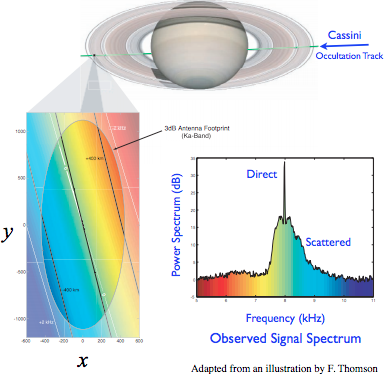
\includegraphics[width=\textwidth]{USER_7a.png}
                	\caption{This is a caption}
                \end{subfigure}
                \begin{subfigure}[b]{0.49\textwidth}
                    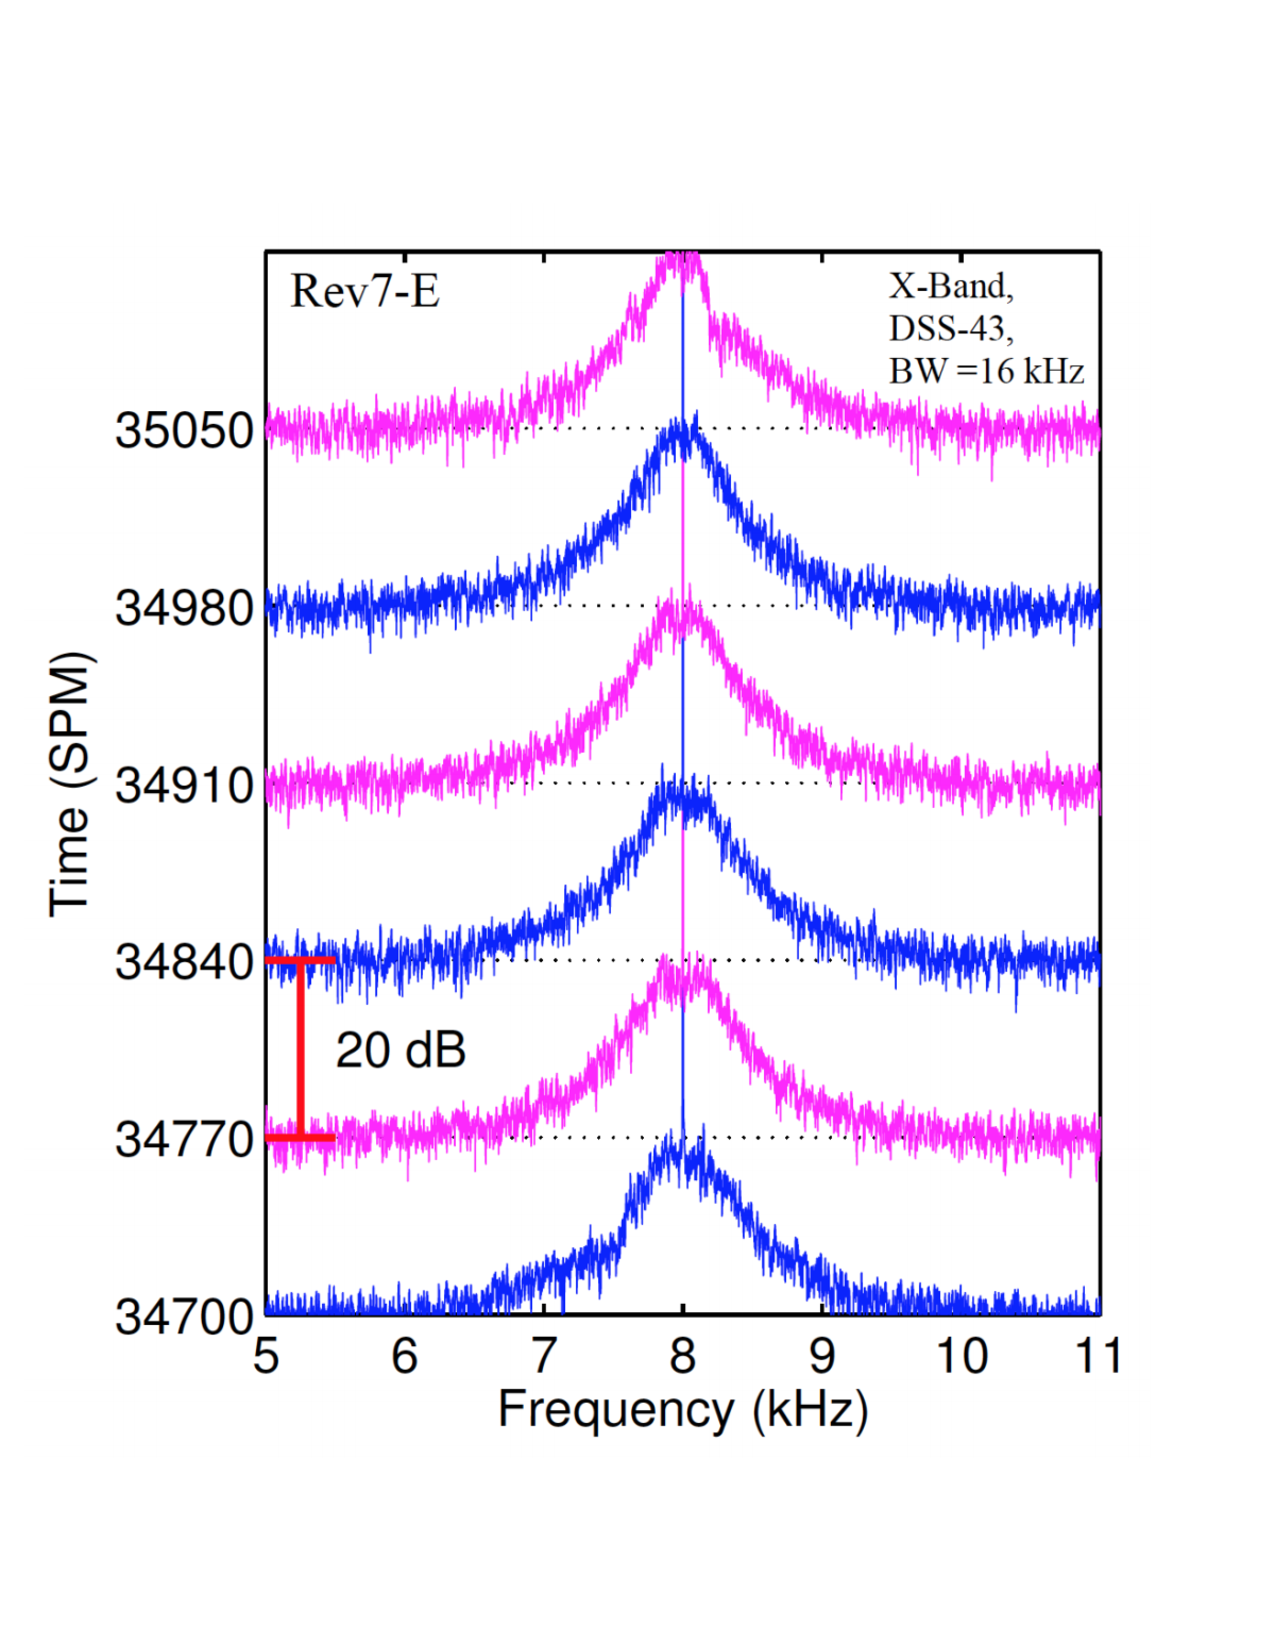
\includegraphics[width=\textwidth]
                        {user_guide_fig_3-9.pdf}
                    \caption{Yadda}
                \end{subfigure}
                \caption{Figures}
                \label{other_label_2}
            \end{figure}
            \noindent As an example, we consider the Cassini egress ring occultation Rev7-E. This image depicts a subset of the power spectra that was derived from the measured $(I_{m}(t), Q_{m}(t))$ samples. Both the direct-to-Earth and scattered signal components are visible. Each spectrum is searched for the frequency of its peak value near the center of the recording bandwidth. The peak is assumed to be the direct signal, but it can be scattered signal or noise where the ring has large optical depth. Least squares fitting of model spectra of sinusoidal signals to the measured spectral values around the peak can be used to refine the position of the peak. $f_{offset}(t)$ is then computed as the offset of the estimated peak frequency from the center of the recording bandwidth $(BW = 1\ \textrm{kHz})$. The first image on the next page depicts the $f_{offset}(t)$ curve computed for Rev-7E. This interval of time covers Rings C, B, and A, as well as free space. Free space is used to form the baseline. The profile is very noisy and almost random in the optically thick regions of Ring B, less noisy in Ring A, and much less noisy in Ring C, the Cassini Division, and outside Ring A. The plot of $f_{dp}(t) - f_{dr}(t)$ is the difference between the reconstructed and predicted Doppler shifts ($f_{dr}(t)$ is the reconstructed, and $f_{dp}(t)$ is the predicted). This accounts for the trend and a large fraction of $f_{offset}(t)$, but not necessary all of it. The difference is $f_{resid}(t) = f_{offset}(t) - \big(f_{dr}(t)-f_{dp}(t)\big)$. Coarser resolution was used to compute this curve to mitigate the effect of noise on the frequency estimates.
            \noindent The most optically thick parts of Ring B yield unreliable estimates. Least squares fit of the reliable parts of the curve yield the heuristic estimate $\hat{f}_{resid}(t)$. Potential causes for $\hat{f}_{resid}(t)$ could be persistent error in the reconstructed spacecraft trajectory and other un-modeled long-term effects. This process is critical for ensuring that the phase of the calibrated signal $I_{c}(t)+iQ_{c}(t)$ is primarily due to ring material, instabilities in the USO reference phase, and any other unknown short-time effects that are no possible to correct for. Reliable computation of ring properties requires accurate determination of the free-space signal level $P_{0}(t)$ used to normalize the signal level through the occultation period. Direct measurement of $P_{0}(t)$ is only possible when the line-of-sight from Cassini to Earth is clear of all rings. Ring occultation observations were designed to allow measurements of $P_{0}(t)$ for a long interval of time exterior to Ring A. The geometry of some radial occultations allowed measurements of $P_{0}(t)$ in the gap between Ring C and Saturn's ionosphere. Least Squares Spline Fitting was used to obtain $P_{0}(t)$ estimates for the ring-free periods. The fitting yields $\hat{P}_{0}(t)$ during the entire observation period. The calibrated, diffraction-limited, complex ring transmittance is defined as:
            \begin{equation}
                \hat{T}_{R}(t)+i\hat{T}_{I}(t)
                =
                \frac{1}{\sqrt{\hat{P}_{0}(t)}}
                \big[I_{c}(t)+iQ_{c}(t)\big]
            \end{equation}
            \begin{figure}[htbp]
            	\centering
            	\captionsetup{type=figure}
            	\begin{subfigure}[b]{0.49\textwidth}
                	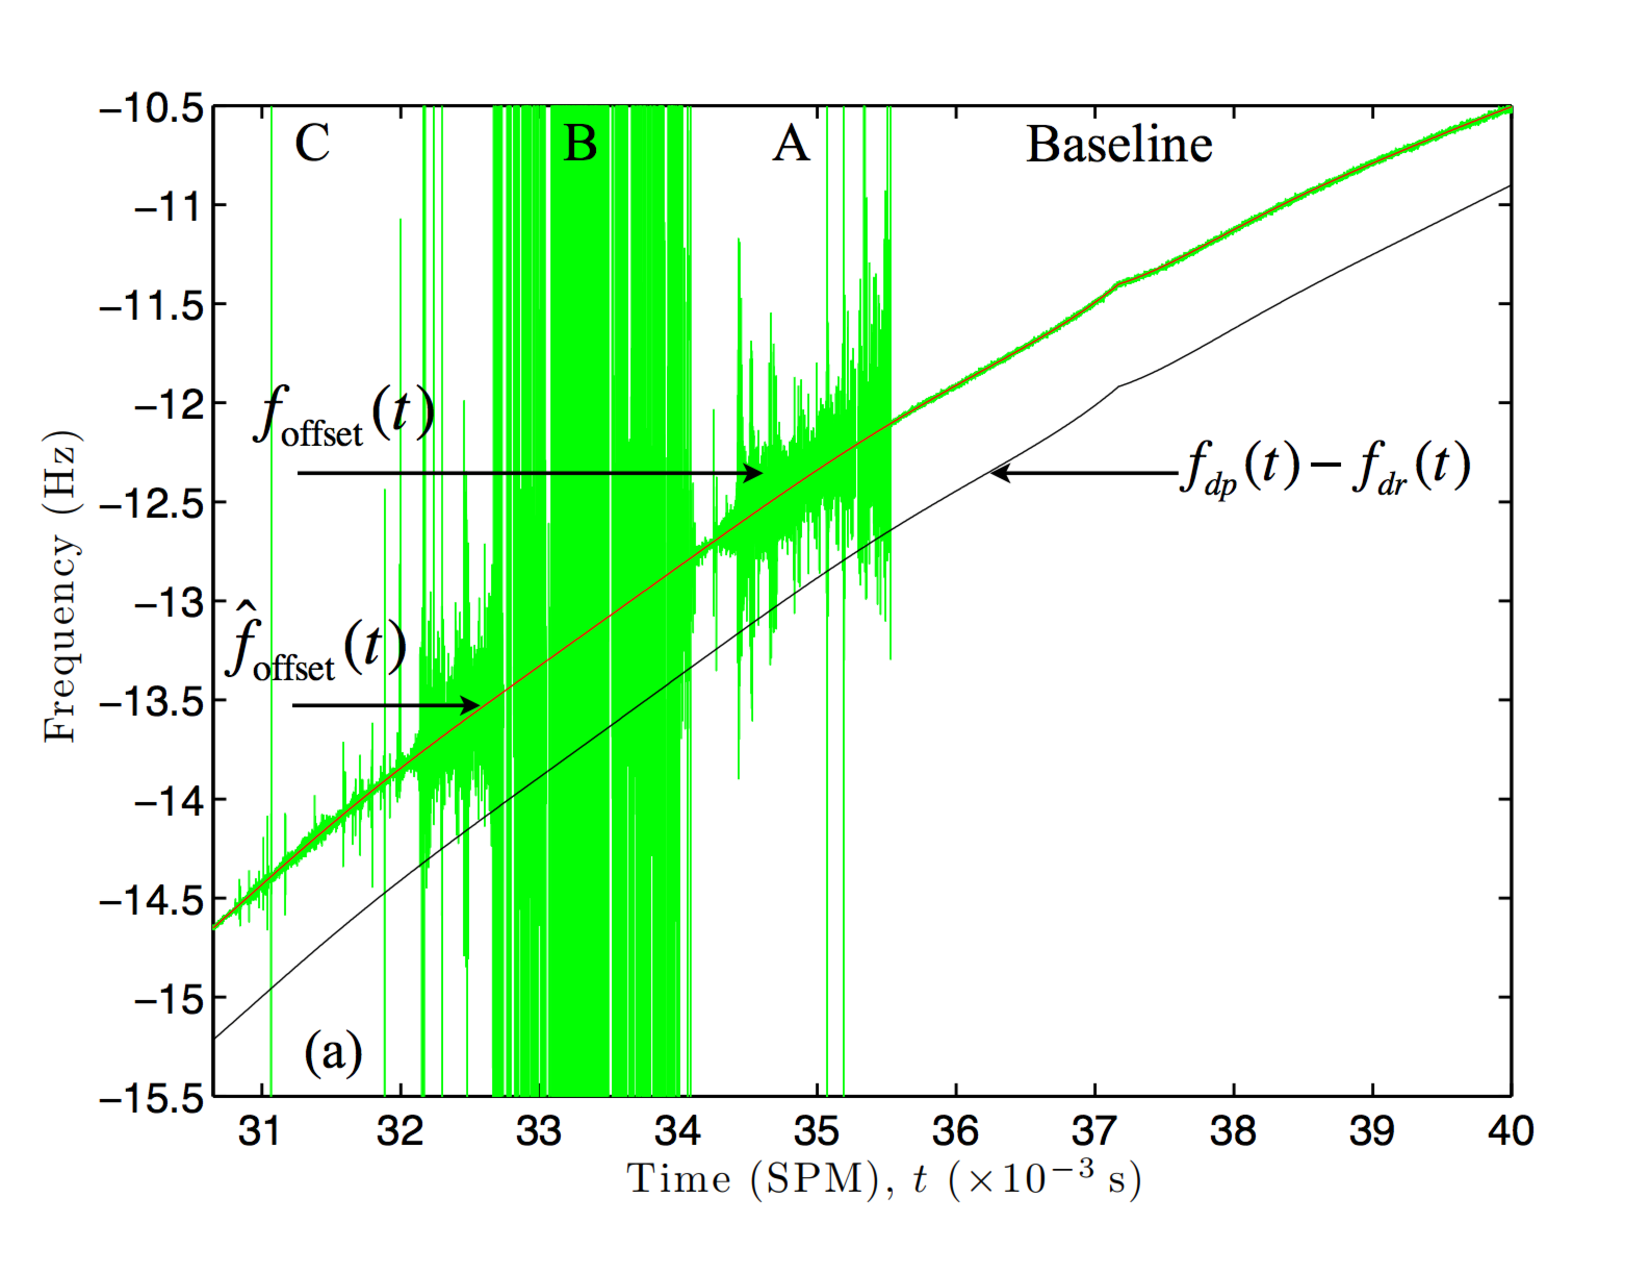
\includegraphics[width=\textwidth]
                	    {user_guide_fig_3-10_a_rotated}
                	\caption{This is a caption}
                \end{subfigure}
                \begin{subfigure}[b]{0.49\textwidth}
                    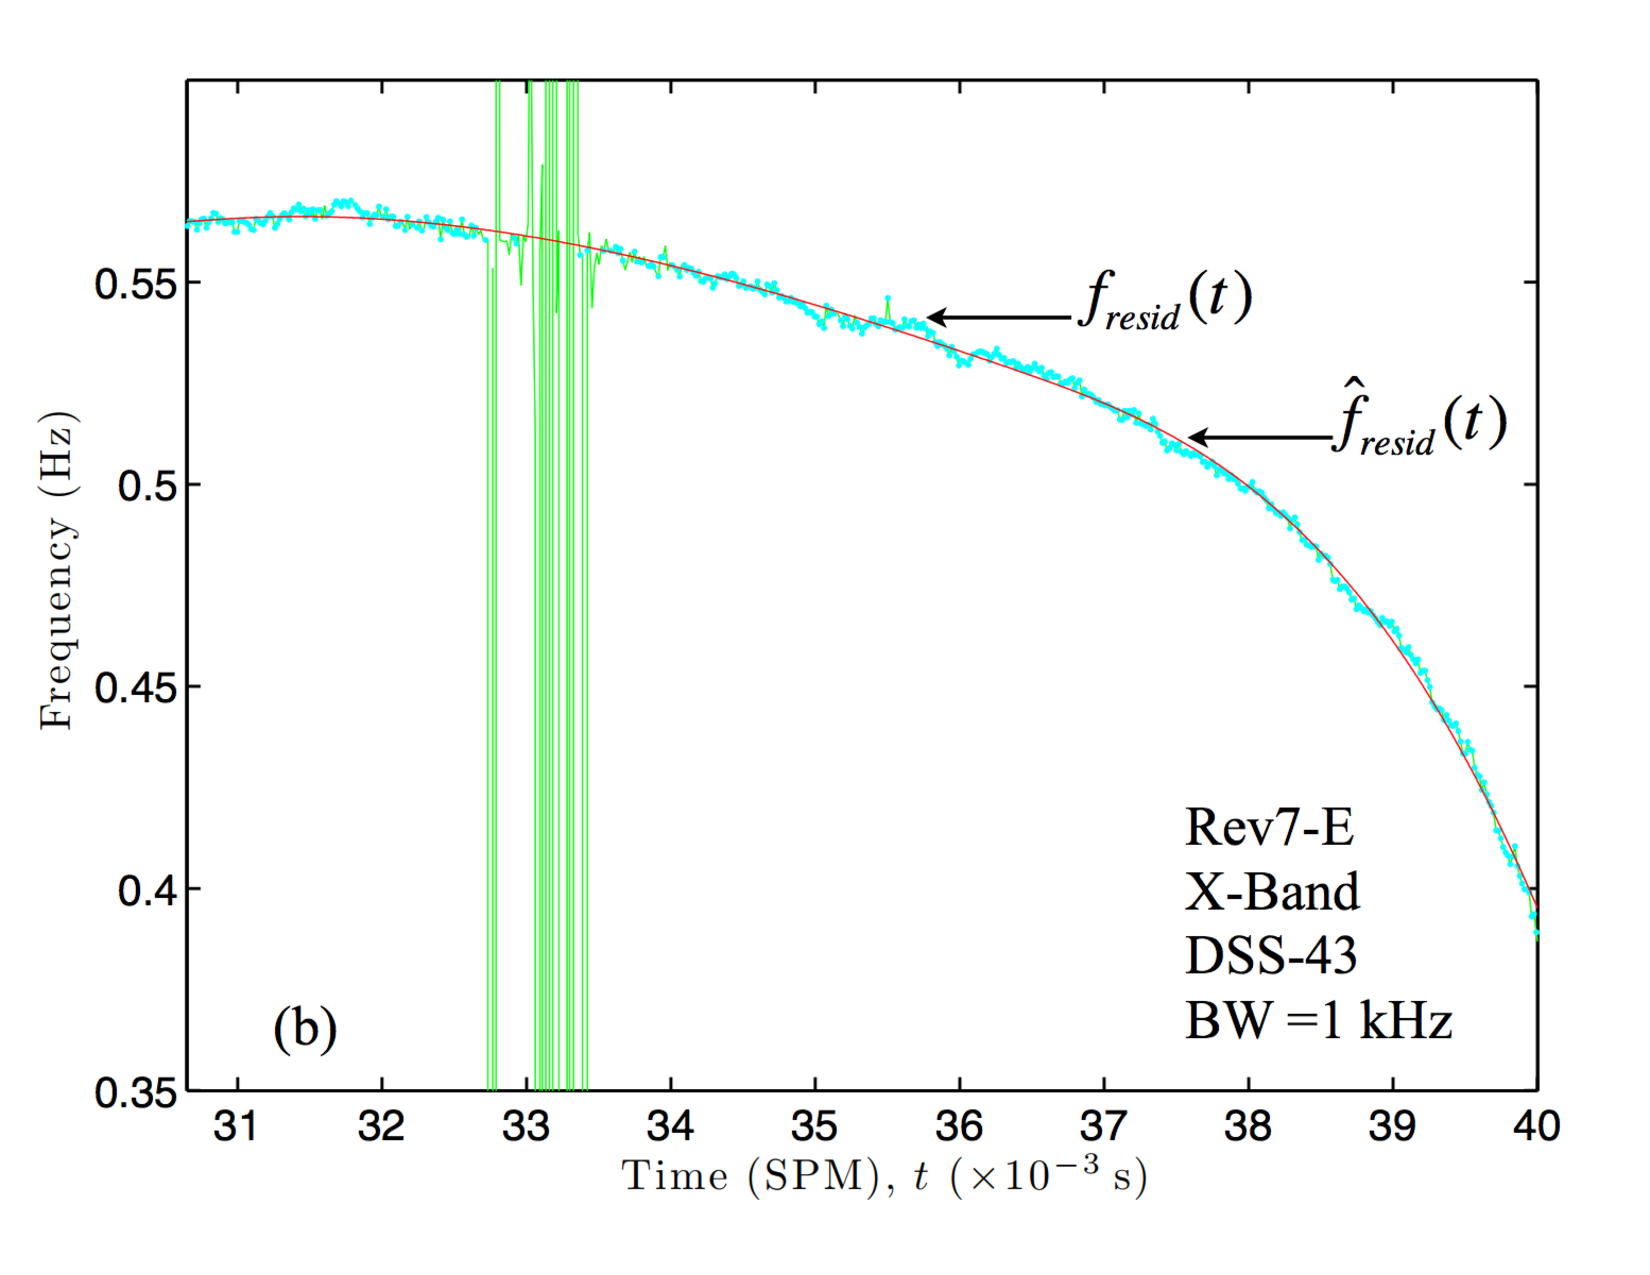
\includegraphics[width=\textwidth]
                        {user_guide_fig_3-10_b_rotated}
                    \caption{Yadda}
                \end{subfigure}
                \caption{Figures}
                \label{other_label}
            \end{figure}
            The calibrated data, $(\hat{T}_{R}(t),\hat{T}_{I}(t))$, form the starting point of all data analysis steps, including computation of optical depth profiles and scattered signal power spectra. There are both short and long term variations in $P_{0}(t)$. Long-term variations are caused by changes in the elevation angle of the DSN receiving antenna during the experiment, and systematic antenna pointing errors. Short-term fluctuations are typically caused by one or more terrestrial factors such as turbulence in the atmosphere, clouds, wind gusts (Causing mechanical vibrations of the receiving antenna), or fluctuations in the receiver gain or thermal noise. Complex samples of the calibrated data are uniformly spaced in time. The below figure depicts estimation of the free-space signal power $P_0(t)$ for Rev-7E.
            \begin{figure}[htbp]
            	\centering
            	\captionsetup{type=figure}
            	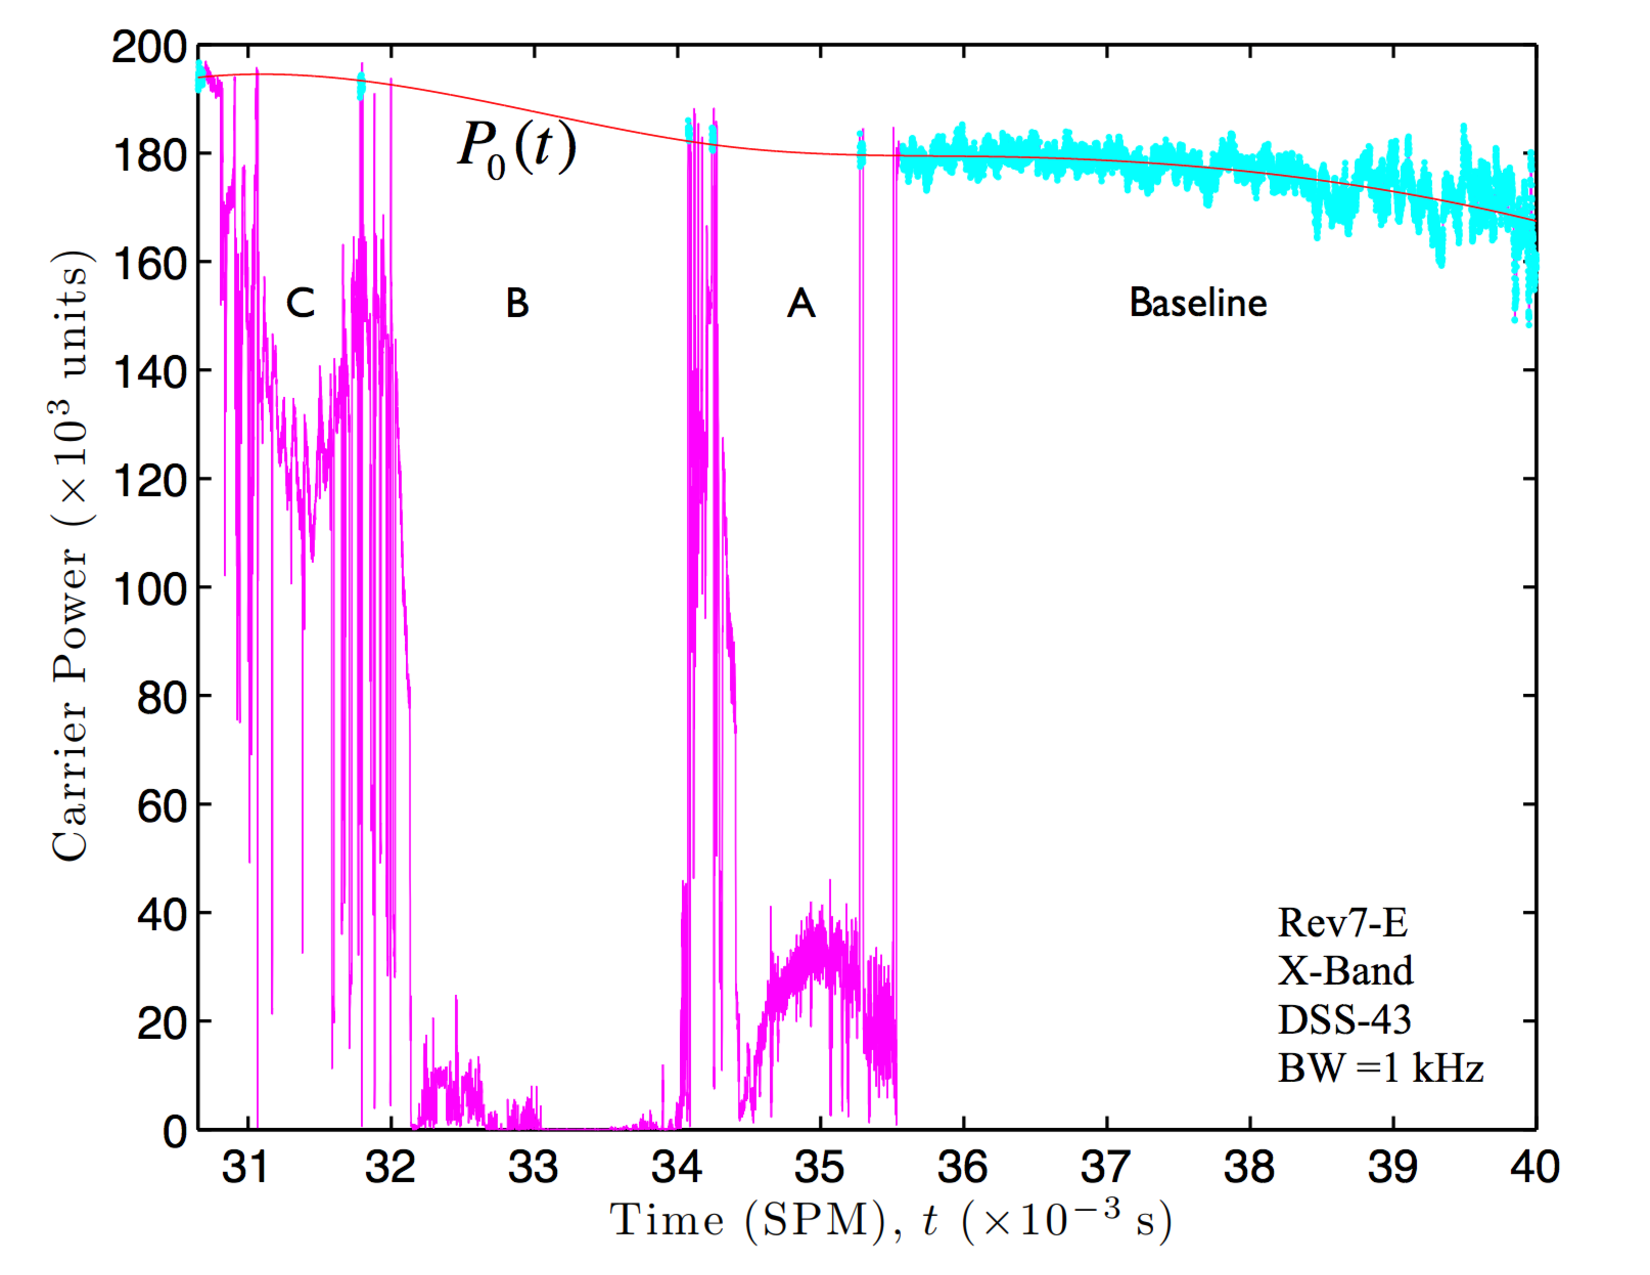
\includegraphics[width = 0.6\textwidth]
            	    {user_guide_fig_3-11rotated2}
            \end{figure}
            The calculations are completed using a quasi-inertial Sun-centered reference frame with the light-time included. Ring accuracy of a few hundred meters is achievable, the primary source of Error being Saturn's pole orientation. The velocity of the ring-plane intercept point varies radially. Data sampled uniformly in time results in non-uniformly samples in ring radius. The following notation is used to denote calibrated complex ring transmittance samples at radius $\rho_0$ where the sampling is uniform in radius:
            \begin{equation}
            \hat{T}(\rho_0) = \hat{T}_{R}(\rho_0)+i\hat{T}_{I}(\rho_0)
            \end{equation}
            
            \noindent Radio occultations observations of planetary rings are diffraction limited. The measured $\hat{T}(\rho_0)$ and the true value of $T(\rho_0)$ differ because of diffraction effects. This difference can be related by the Fresnel Transform.
            
            \begin{equation*}
                \hat{T}(\rho_0) = \frac{1-i}{2F}\int_{-\infty}^{\infty} T(\rho)e^{i\frac{\pi}{2}\big(\frac{\rho_0-\rho}{F}\big)^2}d\rho
            \end{equation*}
            
            \noindent Where $F$ is the Fresnel Scale of Diffraction, which depends on the observation wavelength and geometry. $T(\rho)$ is then:
            \begin{equation}
            T(\rho) = \frac{1+i}{2F}\int_{-\infty}^{\infty}\hat{T}(\rho_0)e^{-i\frac{\pi}{2}\big(\frac{\rho-\rho_0}{F}\big)^2}d\rho_{0}
            \end{equation}
            Quadratic phase approximations, sample resolution of $\hat{T}(\rho_0)$, and signal-to-noise in the measured values set limits on the recovery of $T(\rho)$. The normal optical depth profile and the phase-shift profile are computed as follows:
            \begin{equation*}
                \tau(\rho) = -2\mu_{0}\ln\big(|X(\rho)|\big) \quad\quad\quad\quad \phi(\rho) = \tan^{-1}\bigg[\frac{X_{I}(\rho)}{X_{R}(\rho)}\bigg]
            \end{equation*}
            Where $\hat{X}(\rho_0) = \hat{T}(\rho_0) + \hat{n}(\rho_0)$ and $X(\rho) = T(\rho)+n(\rho) = X_{R}(\rho)+iX_{I}(\rho)$ denote the noisy measured and recovered values, respectively. $B$ is the ring opening angle, and $\mu_0 = \sin\big(|B|\big)$. Practical aspects of the implementation of the Fresnel inversion must be considered. The infinite range of $\rho_0$ must be replaced by the finite data window available. This sets of a limit of $\Delta R_{W} = 2\frac{F^2}{W}$ on the reconstructed resolution, where $W$ is the width of the window. To preserve information about structure on spatial scales equal to or larger than $\Delta R_{W}$, the diffraction-limited data $\hat{T}(\rho_0)$ must be sampled to or larger than twice the highest spatial frequency. This is the sampling theorem. The artificial truncation of the data for a finite width $W$ also creates problems in the reconstruction. To mitigate the sudden jump from positive to zero, a tapered window function that gradually decays to zero may be multiplied by the data. There is a degradation in the spatial resolution by up to a factor of $2$. The Effective resolution is defined below:
            \begin{equation}
            \Delta R_{eff} = -\sim 2\Delta R_{W}
            \end{equation}
            \begin{figure}[H]
                \centering
                \captionsetup{type=figure}
                \begin{subfigure}[b]{0.49\textwidth}
                    \centering 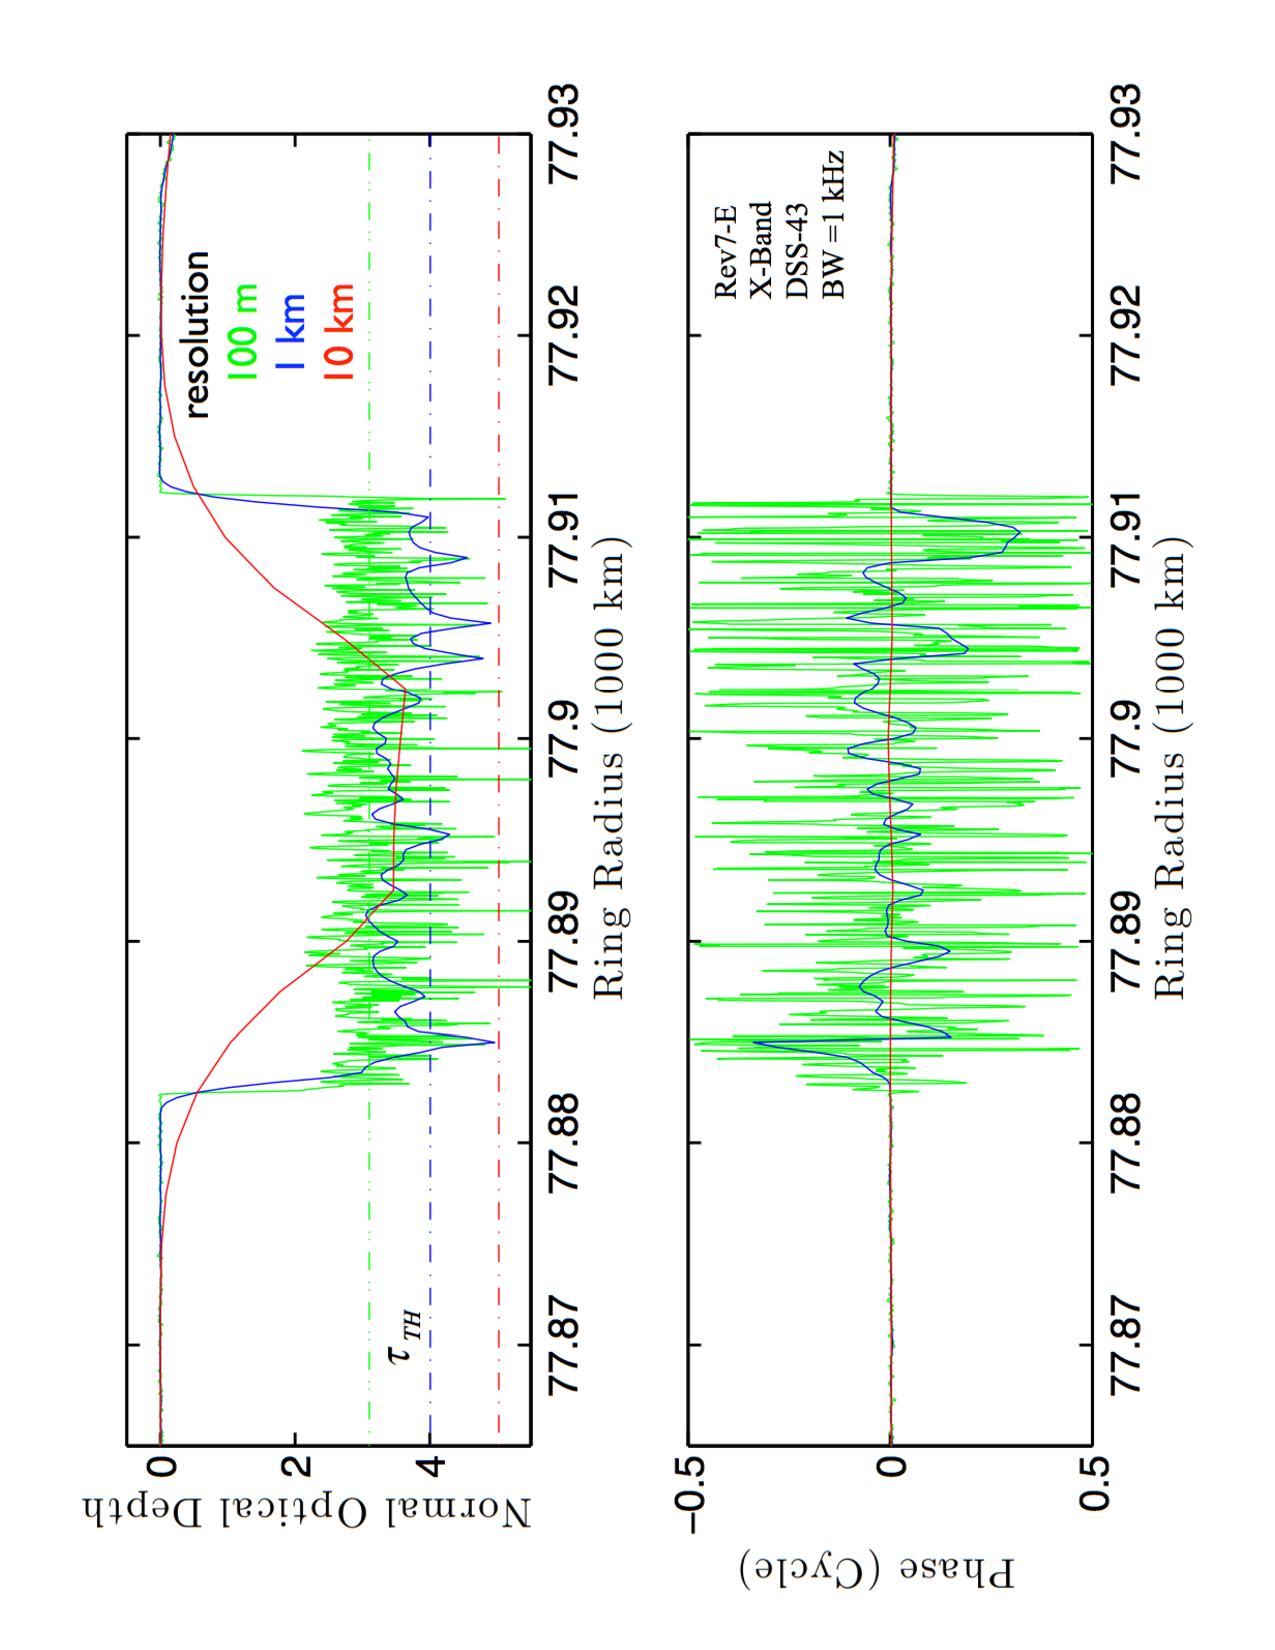
\includegraphics[%
                        angle=-90,
                        width=0.95\textwidth,
                        page=1,
                        trim={0.55in 0.4in 0.55in 0.9in},
                        clip
                    ]{user_guide_fig_3-13.pdf}
                    \caption{CRSUG Fig. 3-13}
                    \label{fig:UGfig3-13}
                \end{subfigure}
                \begin{subfigure}[b]{0.49\textwidth}
                    \centering
                    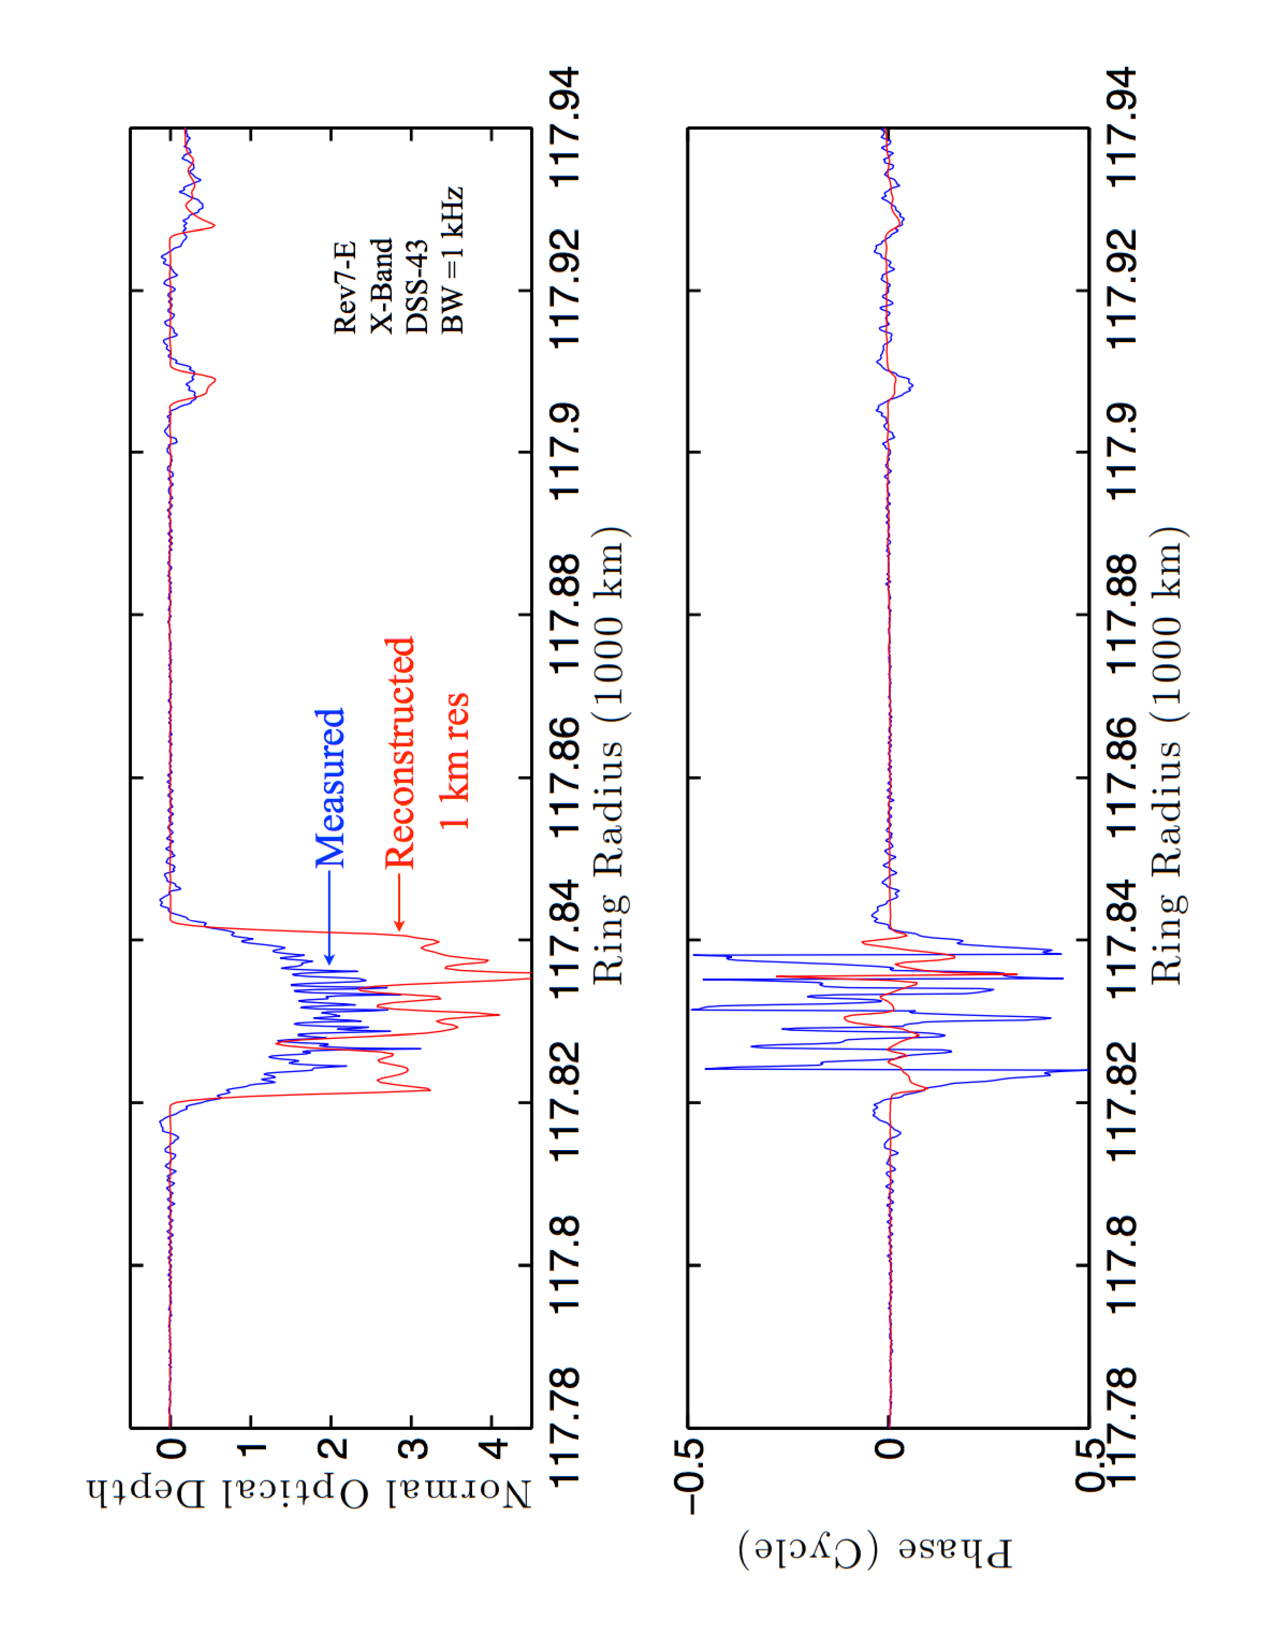
\includegraphics[%
                        angle=-90,
                        width=\textwidth,
                        page=1,
                        trim={0.6in 0.4in 0.6in 0.8in},
                        clip
                    ]{user_guide_fig_3-12.pdf}
                    \caption{CRSUG Fig. 3-12}
                    \label{fig:UGfig3-12}
                \end{subfigure}
                \caption[Titan Ringlet - CRSUG Fig.~3.13]{Optical depth and phase profile reconstructions of the Titan Ringlet.}
                \label{fig:TitanRinglet}
            \end{figure}
            These plots show the diffraction reconstruction of Rev-7E. The main ring feature is the Huygens Ringlet located within the Hugyens Gap. The blue curves represent the diffraction-limited X-band profiles $\hat{\tau}(\rho_0)$ and $\hat{\phi}(\rho_0)$ at 250 m resolution. The red curves depict $\tau(\rho)$ and $\phi(\rho)$ reconstructed using a processing resolution $\Delta R_{W} = 500$ m. The effective resolution is close to $1$ km. The best achievable radial resolution of a given features depends on the optical depth of the feature (The measurement SNR). Finer spatial resolution requires sampling at higher rates, which is noiser. Thermal noise is additive, and the SNR can be improved using coherent averaging. This reduces the resolution. There is thus a trade-off between finer resolution and uncertainty in the reconstructed profile. This is characterized by the threshold optical depth $\tau_{th}$. For a $70\%$ confidence interval:
            \begin{equation}
            \tau_{th} \approx -\mu_0\ln\big(1.205 P_N\big)
            \end{equation}
            Where $P_N$ is the average power of the additive noise. An estimate has the form:
            \begin{equation}
            \hat{P}_N = \frac{1}{SNR_0}\frac{\dot{\rho}_0}{\Delta R}
            \end{equation}
            Where $\Delta R = \Delta \rho_0$, the sample spacing of the diffraction-limited data, or $\Delta R_{eff}$, and $\dot{\rho}_0$ is the ring plane radial velocity of the ring intercept point. For Rev-7E, we have $B = -23.5^{\circ}$ and $\dot{\rho}_0 = 10 \textrm{km/s}$. The images below illustrate the trade-off. $\tau_{th}$ progressively increases from $3.1\rightarrow 4.0 \rightarrow 5.0$ as the resolution of $\Delta R_{eff}$ changes from $100\textrm{m}\rightarrow 1\textrm{km}\rightarrow 10\textrm{km}$. At $100$ m resolution, almost all structure in the ringlet is obscured by noise. The phase profile is essentially random. The ringlet edge is located with high accuracy, though. The absence of profile overshoot in the vicinity of transition to a zero value free-space optical depth indicates reliable reconstruction of the diffraction effects. At fine resolution, diffraction-limited data over a large radial interval is needed to compute the inverse Fresnel transform. 1 km resolution yields more reliable profiling of ringlet structure over the region where the recovered optical depth exceeds the corresponding threshold level, similarly for the phase profile. At 10 km, reliable measurements of the average optical depth of the ringlet is achieved but fine structure is lost. 
            
            \subsubsection{Surface Scattering}
            
            Bistatic radar (BSR) is the active probing of planetary surfaces by oblique reflection and scattering of microwave signals. This provides rms surface slopes and dielectric constant and density at scales comparable to the wavelengths used. A radio signal scatters off the surface and the echo is received on Earth. A direct signal is often sent concurrently. For typical spacecraft transmitters of $1-100$ Watts, surface echoes as low as $1$ Zeptowatt ($10^{-21}$ W) can be detected. Differential Doppler effects between the direct and reflected paths separates the received echo from the carrier. Dispersion of the echo provides a measure of the rms slope of the undulations. Where echo dispersion is small, the Doppler difference between the two primary paths can be used to infer large-scale topography. BSR is interested in amplitude, frequency, polarization, and time of the echo signal. Incremental power from an unresolved surface element is given by:
            \begin{equation}
            dP_{R} = \frac{P_T G_T}{4\pi R_{T}^2}\sigma\bigg(\frac{A_{R}}{4\pi R_{R}^2}\bigg)
            \end{equation}
            $P_T$ is the transmitted power, $G_T$ is the transmitting antenna gain in the direction of the surface element, $R_T$ is the distance from the transmitter to the surface element, $A_R$ is the effective area of the receiving antenna aperture, and $R_R$ is the distance from the surface element to the receiver. The bistatic cross section of the surface element is:
            \begin{equation}
            \sigma = \sigma_{0}dS
            \end{equation}
            Where $dS$ is the area of the surface element, and $\sigma_0$ is the specific radar cross section. $\sigma_0$ is assumed proportional to reflectivity, $\rho$, derived from Fresnel voltage reflection coefficients for horizontally and vertically polarized EM waves at a planar interface between free space and the planetary surface.
            
            \begin{equation}
            R_{HH} = \frac{\cos(\phi) - \sqrt{\epsilon-\sin^2(\phi)}}{\cos(\phi) + \sqrt{\epsilon - \sin^2(\phi)}} \quad \quad
            R_{VV} = \frac{\epsilon \cos(\phi) - \sqrt{\epsilon - \sin^{2}(\phi)}}{\epsilon \cos(\phi) + \sqrt{\epsilon - \sin^2(\phi)}}
            \end{equation}
            
            \noindent Where $\epsilon$ is the dielectric constant of the surface material. The reflection coefficients for circularly polarized waves are:
            \begin{equation}
            R_{SC} = \frac{R_{VV}+R_{HH}}{2} \quad \quad
            R_{OC} = \frac{R_{VV}-R_{HH}}{2}
            \end{equation}
            Where $R_{SC}$ is the voltage reflection coefficient for right-hand circular polarization (RCP) transmitted and received, and $R_{OC}$ is the coefficient for RCP transmitted and Left-Hand Circular Polarization (LCP) received.
            
            \begin{wrapfigure}{l}{0.58\textwidth}
            	\begin{center}
            	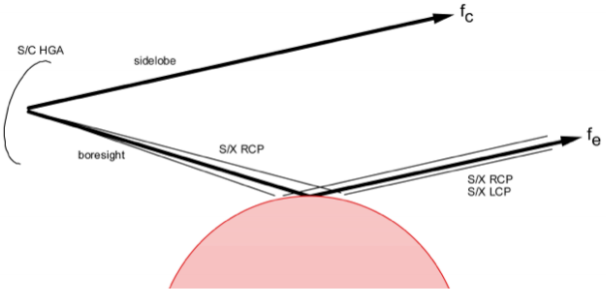
\includegraphics[width = 0.58\textwidth]{USER_12}
            	\end{center}
            \end{wrapfigure}
            \noindent This image depicts the geometry of the experiment. If the transmitter is at $\mathbf{r}_{T}$ and the receiver is at $\mathbf{r}_{R}$, then the Doppler shift is the rate of change of the path length measured in wavelengths $\lambda$. 
            
            \begin{equation}
            f_{c} = \frac{d}{dt}\bigg(\frac{\norm{\mathbf{r}_{T}-\mathbf{r}_{R}}}{\lambda}\bigg)
            \end{equation}
            
            \noindent The Doppler shift for a signal reflected at the point $\mathbf{r}_{P}$ on a smooth target is:
            
            \begin{equation}
            f_{e} = \frac{d}{dt}\bigg(\frac{\norm{\mathbf{r}_{R} - \mathbf{r}_{P}}+\norm{\mathbf{r}_{T}-\mathbf{r}_{P}}}{\lambda}\bigg)
            \end{equation}
            
            \subsubsection{Fundamental Physics}
            
            \noindent GWs are propagating, polarized gravitational fields (Ripples) in the curvature of space-time. Such waves are predicted by all relativistic theories of gravity. These waves are propagating space-time strain. They cause fractional frequency shifts of electromagnetic waves exchanged between separated test mass and cause differences in the rates at which separated clocks keep time. GWs are propagating solutions of Einstein's Field Equations. They propagate at the speed of light, carry energy and momentum, are transverse to the propagation direction, and have two independent polarization states. GWs couple very weakly to matter. Only massive sources undergoing extreme dynamics could generate detectable waves. This means GWs preserve information about the deep interiors of high gravity/high velocity objects. The Doppler tracking method measures the Earth-Spacecraft fractional Doppler shift, $\frac{\delta f}{f_0}$, where $\delta f$ is the Doppler shift and $f_0$ is the radio link's carrier frequency. The Doppler shifts due to Earth and spacecraft motion must be removed, the ODP is used for this. The difference between observed sky frequency and predicted sky frequency is called the residual frequency. Dividing this by the link center frequency, $f_0$, gives the value of $y$. The GW signature in the time series is:
            \begin{equation}
                y_{signal}=\frac{\mu-1}{2}Y\big(t\big)-
                           \mu Y\big(t-\frac{1+\mu}{2}T_2\big)
                          +\frac{1+\mu}{2}Y\big(t-T_2\big)
            \end{equation}
            Where $\mu$ is the cosine of the angle between the
            Earth-spacecraft line and the propagation vector of the GW, $Y(t)
            = \frac{\hat{\mathbf{n}}\cdot \mathbf{h}}{1-\mu^2}$, where
            $\hat{\mathbf{n}}$ is the unit vector from Earth to the
            spacecraft, and $\mathbf{h}$ is the first order metric
            perturbation of the Earth. This response of the Dopple to a GW
            excitation is interpreted as due to the GW striking the Earth, the
            GW striking the spacecraft (at a delayed time), and the original
            Earth buffeting transponded back to the Earth a two-way light time
            later. The parametrized Post Newtonian (PPN) formalism is a formal
            approach to compare metric theories of relativistic gravity with
            each other and with experiments. The PPN approach is simplest in
            slow motion, weak field limits. In the inner solar system,
            $\norm{\mathbf{v}}$, the velocity of an object with respect to the
            center, is usually less than 30 km/sec. So $\frac{v^2}{c^2}
            \approx 10^{-8}$, and this is considered slow. At the surface of
            the Sun, $\frac{U}{c^2}$, where $U$ is the Newtonian potential, is
            on the order of $10^{-6}$. Everywhere else in the solar system is
            much less. So, the PPN is simple for the solar system. The
            parameter $\gamma$ characterizes the space-time curvature produced
            per unit mass. In the Theory of General Relativity (GR),
            $\gamma=1$. $\gamma$ has been measured by measurements of the
            range and range rate between Earth and distant spacecraft as the
            line between the two passes close to the Sun. Non-Newtonian
            contributions from the Sun's curving of space-time are created. 
            \begin{equation}
            \Delta t=\frac{1+\gamma}{2}
                \bigg(240- 20
                    \frac{\ln\bigg(\frac{b^2}{r_{sun}^2}\bigg)}
                         {\frac{r}{1\textrm{AU}}}\bigg)
            \end{equation}
            Where $b$ is the impact parameter of the ray, $r_{Sun}$ is the
            solar radius, and $r$ is the range to the spacecraft. Viking range
            observations had $\gamma=1$ to one part in $1000$. For Cassini,
            the radial velocity was measured. Due to motions of the spacecraft
            and the Earth during the conjunction, the closest approach
            distance changes with time, inducing a relative frequency shift of
            the carrier:
            \begin{equation}
                \frac{\Delta v}{v}=-\frac{d\Delta t}{dt}
                                  =-4(1+\gamma)\frac{GM}{bc^3}\frac{db}{dt}
                                  =-2\mu s(1+\gamma)\frac{1}{b}\frac{db}{dt}
            \end{equation}
            In 2002, Cassini was 7.4 AU from the sun. $\frac{db}{dt}$ was
            close to being determined by the Earth orbital velocity, and the
            relative frequency shift was on the order of $10^{-9}$. Radio
            signals are strongly affected by the solar corona. The refractive
            index of the spectrum is inversely proportional to the square of
            the carrier frequency, and thus $X$ and $Ka-$band signals were
            nearly completely free of these plasma effects.
\end{document}